% !TEX root = ../rawlik-phd-thesis.tex
\chapter{Coil design} % Chapter title
\label{ch:coil_design}

This is largely based on the publication \note{cite here the AJP publication, once it's out.}

\section{Introduction}
How to design a coil, or more generally, an arrangement of coils, producing a desired magnetic field? The problem is surprisingly hard and the solutions, how the wire making up the coil should be laid, complicated. The most widespread application of high--performance coils is Magnetic Resonance Imaging (MRI), where gradient coils give the possibility to produce spatial images. Already in the 1980's elaborate methods of MRI coil design have been developed. They range from optimizing positions of discrete windings, where use is made of symmetries specific to MRI, to analytical methods yielding surface current density, which is then discretized. A general overview can be found in \cite{Turner1993}. Another field known for complex, precise coils is plasma--confinement, in particular stellarators \cite{Beidler1990}. There analytical solutions for the surface current density find their use, too.

% Suggest problems:
% 6.55
% One way to produce a very uniform magnetic field is to use a very long solenoid and work only in the middle section of its interior. This is often inconvenient, wasteful of space and power. Can you suggest ways in which two short coils or current rings might be arranged to achieve good uniformity over a limited region? Hint: Consider two coaxial current rings of radius a, separated axially by a distance b. Investigate the uniformity of the field in the vicinity of the point on the axis midway between the two coils. Deter- mine the magnitude of the coil separation b that for given coil radius a will make the field in this region as nearly uniform as possible.
% 6.62
% For a delicate magnetic experiment, a physicist wants to cancel the earth’s field over a volume roughly 30 × 30 × 30 cm in size, so that the residual field in this region will not be greater than 10 milli- gauss at any point. The strength of the earth’s field in this location is 0.55 gauss, making an angle of 30◦ with the vertical. It may be assumed constant to a milligauss or so over the volume in question. (The earth’s field itself would hardly vary that much over a foot or so, but in a laboratory there are often local perturbations.) Deter- mine roughly what solenoid dimensions would be suitable for the task, and estimate the number of ampere turns (that is, the current I multiplied by the number of turns N) required in your compen- sating system.

We would like to present a method that may not be competitive when it comes to precision, but is distinct in its simplicity, also when it comes to construction of its designs. It relies on an algebraic representation of the problem, where coil design is simplified to a simple linear least squares problem. In our method the coils are restricted to a user--defined mesh, making it easy to deal with spatial constraints.

% The method has been originally developed to design coils of the active magnetic field stabilisation system of the neutron electric dipole moment (nEDM) experiment at the Paul Scherrer institute in Villigen, Switzerland. This application, which we discuss later in the paper, requires many large (5--7 meters) coils. In the presented method the arrangements of coils are designed on a predefined grid. This makes the construction of even complicated coils feasible, despite the size. Firstly, all coils can be designed to share the grid, and secondly, the grid can be defined such, that it avoids conflicts with the experimental apparatus.

Here would come a paragraph Klaus suggested: For the second one, I would suggest that you add an explicit paragraph to set the scene and
spell out what we expect, e.g., the ‘undergraduate student’ to know, i.e. how to calculate
a field from a finite current, how to superimpose fields from many currents, as well as
how to solve  a system of linear equations. You could mention these things and refer to
two typical undergraduate text books. You can then explain that there is an elegant 
and understandable solution presented in the available source code [ref].

The method has originally been developed to design coils of the active magnetic field stabilization system of the neutron electric dipole moment (nEDM) experiment at the Paul Scherrer Institute in Villigen, Switzerland. This application, described in detail in \cite{Afach2014}, which we discuss later in the paper, requires large (6--8 meters side length) coils. In the presented method the coil systems are designed on a predefined grid. This makes the construction of even complicated coils feasible, despite the size.

% \note{Maybe try to write more \emph{why} is the problem in general case so difficult, and what is so special in this method that makes it simple?}

% In active magnetic field stabilisation systems the desired field shape is not even known beforehand -- a system capable of producing an arbitrary field is desired.

% In particular finds use in active magnetic field stabilisation systems, eg. in nEDM experiments or in PTB \note{(really?)}.

% An interesting approach to coil design was presented by \cite{Compton1982}. He proposed to divide a surface into small elements and solve for current density in each element. This is very general and powerful idea, albeit the solution is likely to be hard to build.

% Most of modern coil design approaches focus on increasing the precision of the created field, giving designs that are very difficult to manufacture. The presented approach focuses on versatility and ease of practical realisation, which makes it potentially useful for large scale builds and systems employing multiple coils.

% Mention the main feature of this approach --- the spatial constraint on the location of the wires? Needs some explanation probably.

% \note{Mention the mechanical restriction of the method?}

We begin with a description of our model in a restricted 2-dimensional case and generalize it to three dimensions. We then present how the model is used to design a coil, based on an example. Further we discuss possibilities of simplifying the solution. Another section is devoted to practical considerations, significant for the eventual construction. Finally, we analyze the design method in the particular case of the magnetic field stabilization system of the nEDM experiment at the Paul Scherrer Institute.


\section{Coils as a linear space}
Consider all possible coils that can be constructed by laying a wire on a surface of a square. The possibilities are endless. Speaking more precisely, as the wires may be shifted by arbitrarily small distances, as they overlap and cross, the problem has inherently an infinite number of degrees of freedom. We present an algebraic representation that reduces the number of degrees of freedom to just a few.

We start with a finite wire segment carrying current $I$, spanned between points $\bm{x}_1$ and $\bm{x}_2$ (represented by vectors in an arbitrary coordinate system), as depicted in Fig.\,\ref{fig:biot-savart}. To calculate the magnetic field it produces in the point $\bm{p}$ we consider the vector normal to the wire through the point $\bm{p}$:
\begin{equation}
  \bm{\rho} = (\bm{x}_1 - \bm{p}) - \left( \left( \bm{x}_1 - \bm{p} \right) \cdot \bm{n} \right)\bm{n} \ ,
\end{equation}
where $\bm{n}$ is a unit vector in the direction $\bm{x}_2 -\bm{x}_1$. The magnitude of the magnetic field in point $\bm{p}$ is then \cite{Griffith}:
\begin{equation}
  \label{eq:biot_savart}
  B = \frac{\mu_0 I}{4 \pi \rho} \, \left| \sin \alpha_2 + s\, \sin \alpha_1 \right| \ ,
\end{equation}
where the angles $\alpha_i$ are not directed:
\begin{equation}
  \alpha_i = \frac{ \left| \bm{x}_i \times \bm{\rho} \right| }{ x_i \rho } \ ,
\end{equation}
and $s$ is $+1$ if $\bm{\rho}$ points onto the wire segment (between points $\bm{x}_1$ and $\bm{x}_2$) and $-1$ otherwise:
\begin{equation}
  s = \mathrm{sgn}\left( \left| \bm{x}_2 - \bm{x}_1 \right| - \left| \bm{p} + \bm{\rho} - \left( \bm{x}_1 + \bm{x}_2 \right) / 2 \right| \right)
\end{equation}
The direction of the field is given by the right-hand principle:
\begin{equation}
  \mathbf{B} = \frac{B}{\rho} \bm{\rho} \times \bm{n}
\end{equation}
This formulation is independent on the coordinate system (coordinate-system dependent solutions can be found e.g.\ in \cite{Grivich2000}).

% (x1 .- p) .- ((x1 .- p) ⋅ n) * n

\begin{figure}
  \centering
  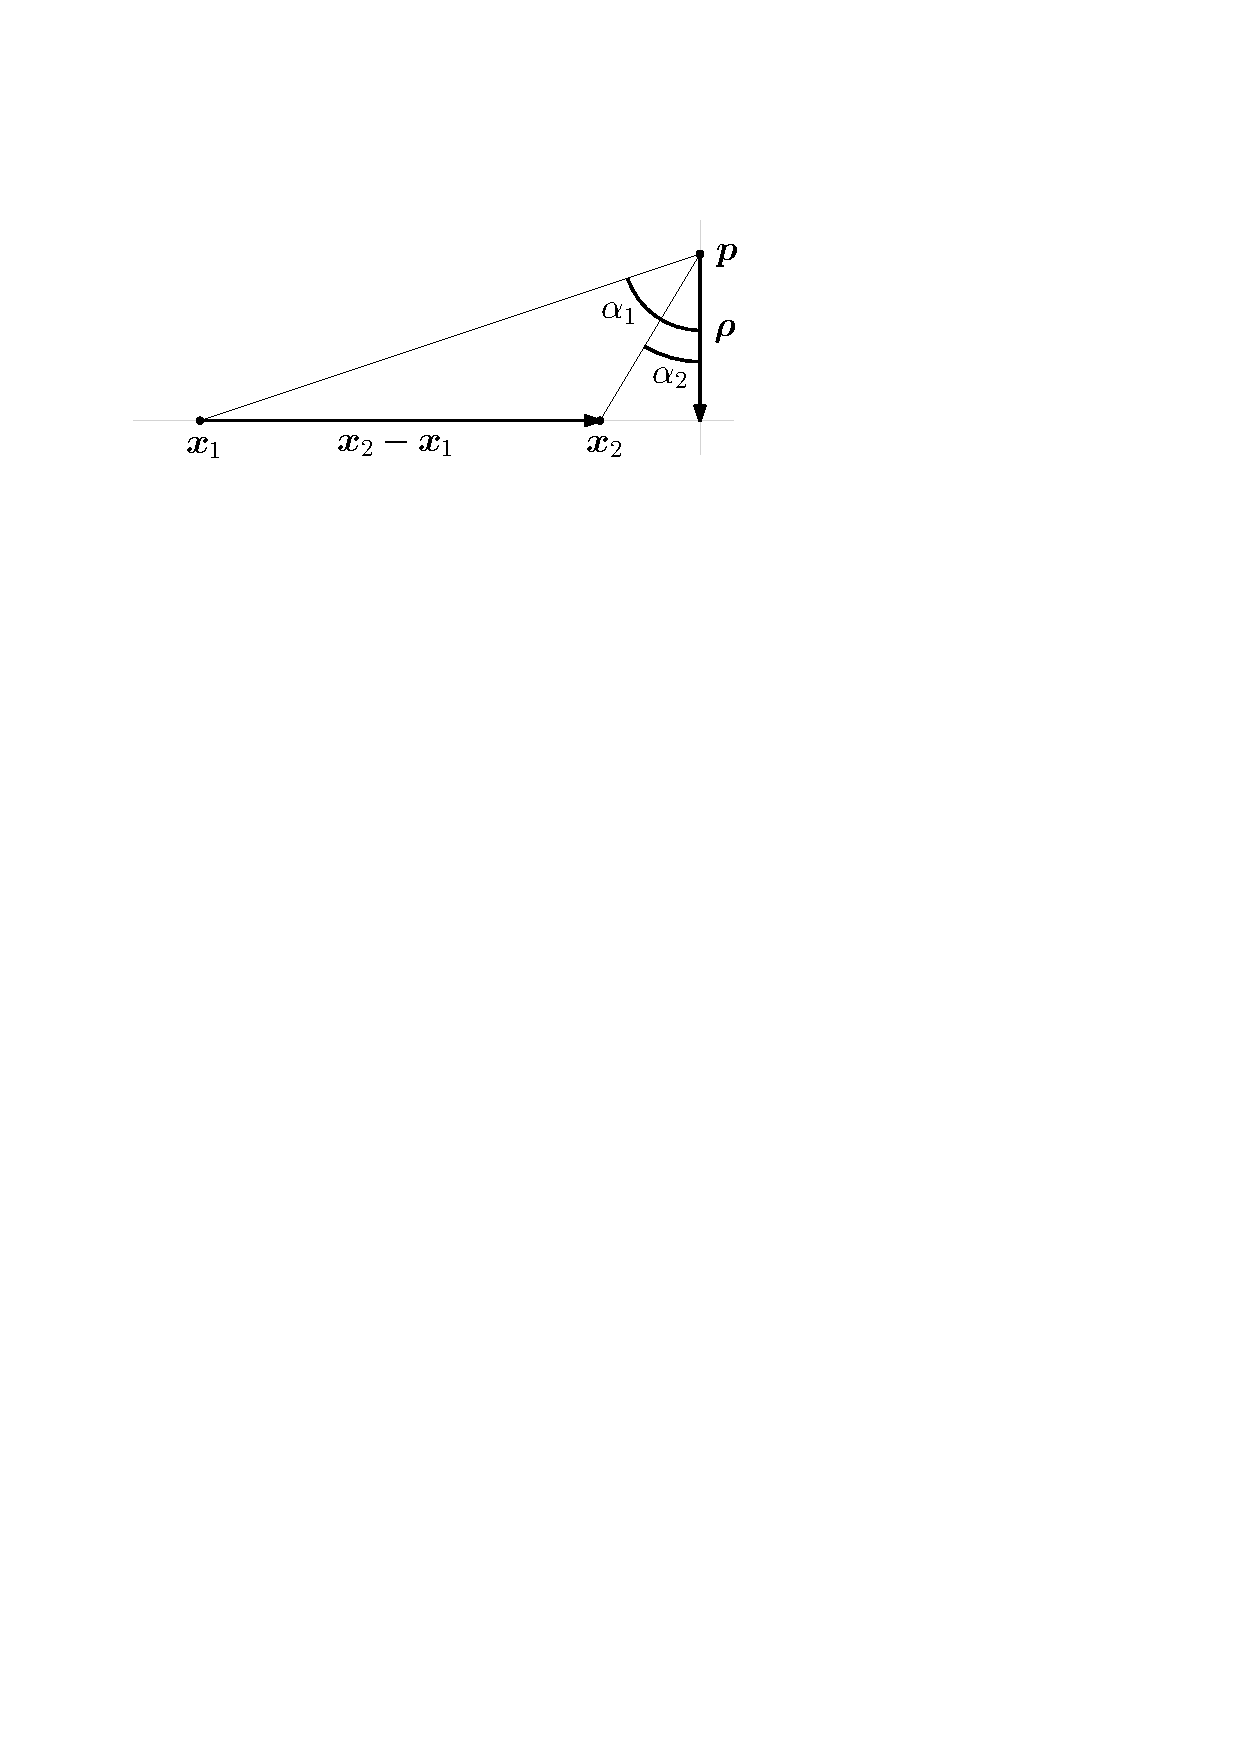
\includegraphics[width=0.8\linewidth]{gfx/coils/biot_savart.pdf}
  \caption{The setting for calculating the magnetic field produced in point $\bm{p}$ by a straight wire segment from $\bm{x}_1$ to $\bm{x}_2$.}
  \label{fig:biot-savart}
\end{figure}

Let us imagine a square loop of a wire with a current flowing through it -- a coil. It produces a certain magnetic field in the entire space $\mathbf{B}(\mathbf{x})$, given, following the superposition principle, by a sum of the fields produces by each segment of the coil. 
By changing the current in the coil we alter only one parameter of the magnetic field -- the magnitude, but not its shape. It can therefore be said that one coil spans a one--dimensional space of magnetic fields it can produce. Adding a second, different coil creates a system spanning a two--dimensional space of fields, as the magnetic field is additive. Going a step further, four square coils tiled to form a larger square form a four--dimensional space, as shown in Fig.\,\ref{fig:coils_tile_basis}. Any coil restricted to the $2 \times 2$ grid can be represented in the base of the four tile--coils.

The range of magnetic field reachable by coils restricted to a grid is a subset of all possible fields that can be created with coils constructed on the square's surface. The size of the subset is controlled by $N$, the number of tile--coils forming the grid.
% It is worthwhile to note that, in fact, a coil is equivalent to the field it produces . By constructing the grid we have thus restricted ourselves to a subset of \emph{coils} that are possible to construct on the square.
In this system a coil is fully described by a vector of $N$ currents, one in each of the tile--coils, denoted by $\mathbb{I}$. The problem of coil design is thereby simplified to finding a vector $\mathbb{I}$.
% The four coils form a complete linear basis of coils on the surface for any coils that have wires going only along the edges --- see Fig.\,\ref{fig:coils_tile_basis}. This is a very convenient subspace of all coils possible to build on a square. The possible to realise subspace may be enlarged by refining the division into tiles. But as a coil is equivalent to the field it produces, one can just as well say that they form a four--dimensional \emph{space of coils}.

\begin{figure}
  \centering
  \includegraphics[width=0.8\linewidth]{gfx/coils/tile_basis.pdf}
  \caption{a) A basis of four tile coils on a flat square. Any coil which has its wires restricted to lie on the $2 \times 2$ grid can be represented as a linear combination of the four base tile coils. b, c, d) Three coils are presented together with their explicit coordinates in the basis.}
  \label{fig:coils_tile_basis}
\end{figure}

Generalisation onto a cube is simple, a cube being made up of six square faces. Interestingly, in the assembly in a three--dimensional space one degree of freedom is lost.  Figure~\ref{fig:coils_tile_kernel} illustrates, in the simplest case $N = 6$, a configuration in which finite currents in all six coils cancel and no magnetic field is produced. Such a combination of currents can be added to any solution with no effect on the produced field. Effectively, the space of the fields they can produce has dimension 5 ($N-1$). In other words, the mapping of $\mathbb{I}$ onto fields $\mathbf{B}(\mathbf{x})$ has in this case a one--dimensional kernel. This fact is of importance when it comes to numerically solving the system.

\begin{figure}
  \centering
  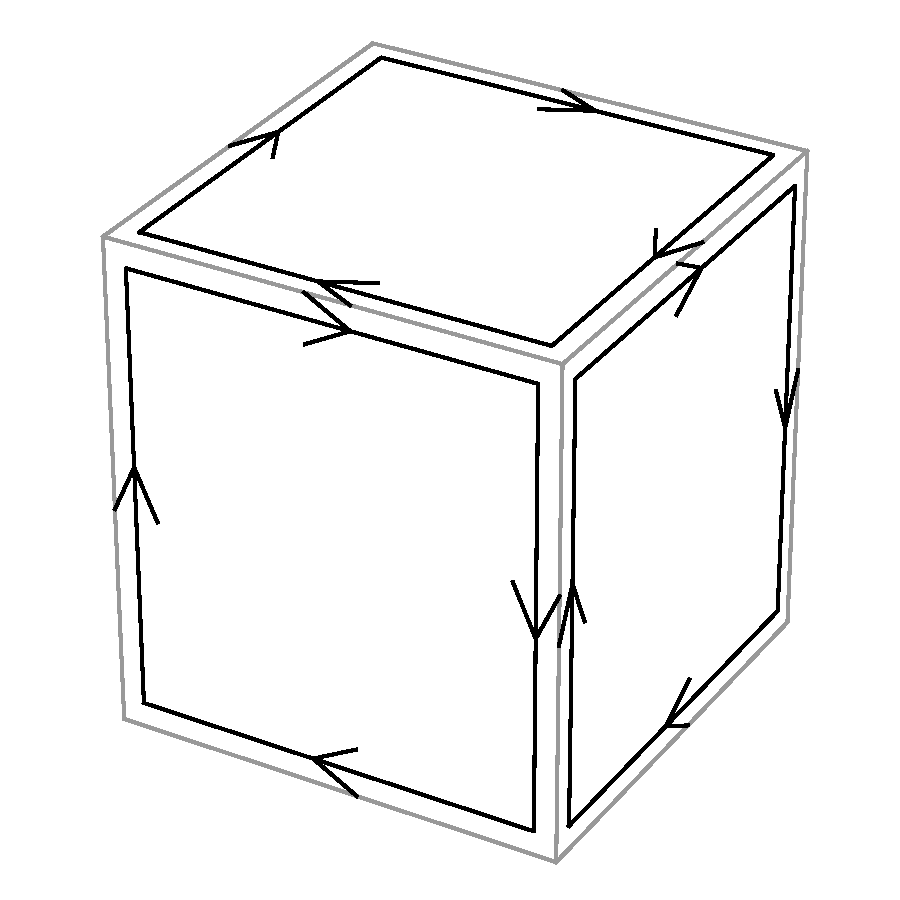
\includegraphics[width=0.5\linewidth]{gfx/coils/tile_kernel2.pdf}
  \caption{An arrangement of $N = 6$ tile coils on a cube which produces no magnetic field. The currents in the tiles are equal and flow in the directions as indicated. The currents on the invisible faces are analogous to the ones seen in front. For clarity, the coils are depicted slightly smaller; in the model the currents are identical with the edges of the cube.}
  \label{fig:coils_tile_kernel}
\end{figure}

This is the foundation of the method. We restrict ourselves to a grid on a cuboid, but in return we can fully describe all coils in the restricted space by a vector of $N$ numbers.

% Consider six square coils combined into a cube form only a five--dimensional space of coils, as same current flowing in each of the coils, in opposite directions for adjacent faces, produces no field. This is visualised in Fig.\,\ref{fig:coils_tile_kernel}. Dividing the faces of the cube into $N$ tiles provides a simple basis for many coils that can be built around a volume. This being the case of most practical interest, we will be further considering a cube.

% A cube consists of six square faces. On each a grid may be constructed, forming a set of $N$ \emph{base coils}.  smaller The problem of coil design is much simpler, as now it is a problem in a finite--, $N$--dimensional linear space. A $coil$ is fully described by a set of $N$ currents in each of the \emph{base coils} --- $\mathbb{I}$. At the cost of restraining oneself to coils that can have wires only along the edges of the tiles, one gains a tremendous simplification of the problem.
% However, six square coils combined into a cube form only a five--dimensional space of coils, as same current flowing in each of the coils produces no field, as explained in Fig.\,\ref{fig:coils_tile_kernel}. Dividing the faces of the cube into $N$ tiles provides a simple basis for many coils that can be built around a volume.


%   \quad
%   \subfloat[A coil which spans one--dimensional subspace of coil--vectors on a cuboid that produces no magnetic field.]
%   {\label{fig:coils_tile_kernel}
%   \includegraphics[width=.45\linewidth]{tile_kernel}}
%   \caption{Coils as a vector space.}
% \end{figure}
%
% \begin{figure}[bth]
%   \centering
%   \subfloat[A basis of four base--coils on a surface. Three vectors are presented together with their explicit coordinates in the basis.]
%   {\label{fig:coils_tile_basis}
%   \includegraphics[width=.45\linewidth]{tile_basis}}
%   \quad
%   \subfloat[A coil which spans one--dimensional subspace of coil--vectors on a cuboid that produces no magnetic field.]
%   {\label{fig:coils_tile_kernel}
%   \includegraphics[width=.45\linewidth]{tile_kernel}}
%   \caption{Coils as a vector space.}
% \end{figure}


\section{Coil design}
In the problem of coil design one wants to create a coil, or an arrangement of coils, which best approximates a given field in a certain volume, which we will call \emph{the volume of interest}. Rather than considering the whole volume, we pick an ensemble of $m$, points of interest on its surface (the surface is sufficient because $\nabla \cdot \mathbf{B} = 0$). Hence, we look at the magnetic field $\mathbf{B}(\mathbf{x})$ only at these points and gather the values $\mathbf{B}(\mathbf{x}_i)$ for $i = 1 .. m$ into a vector of dimension $3m$ ($B_x$, $B_y$ and $B_z$ in each point), which we shall denote $\mathbb{B}$.

% Note, that magnetic field produced by a coil at a given point in space is proportional to the current in this coil. For a fixed direction in a fixed point in space it is a linear combination of currents of all coils in the system. Now, if we consider a vector of 3 spatial directions in $M$ points \ie, dimension $3M$. It can be obtained from an arbitrary coil $C$ by multiplying it by a $NNN \times 3M$ matrix $\mathbb{M}$. This matrix encodes the geometry of the system and may be pre-calculated.

As mentioned before, the magnetic field produced by a coil at any given point in space is proportional to the current in this coil. With many coils present it is a linear combination of the currents of all coils in the system. In absence of an external magnetic field the system of $N$ tiles and $m$ points of interest is thus described by a simple linear equation:
\begin{equation}
  \label{eq:matrix}
  \mathbb{B} = \mathbb{M} \, \mathbb{I}
\end{equation}
where $\mathbb{M} \in \mathbb{R}^{3 m} \times \mathbb{R}^{N}$ is a matrix of proportionality constants. For example, the element $\mathbb{M}_{(5, 2)}$ is the proportionality constant between the current in the second of $N$ coils and the magnetic field in the $y$ direction in the second of $m$ points of interest, $B_x(\mathbf{x}_1)$. The matrix $\mathbb{M}$ can be calculated analytically using the Biot--Savart law.

Equation~(\ref{eq:matrix}), for $3m > N - 1$, is an over--determined set of linear equations, $\mathbb{I}$ being the vector of unknowns. We look for the optimal least--squares solution $\mathbb{I}_0$ to produce a $\mathbf{B}_0(\mathbf{x})$ in the volume of interest:
\begin{equation}
  \label{eq:requirement}
  % \mathbb{M} \, \mathbb{I} \stackrel{!}{=} \mathbb{B}_0
  \mathbb{I}_0 = \mathrm{arg}\,\min_{\mathbb{I}} \left( \mathbb{M} \mathbb{I} - \mathbb{B}_0 \right)^2 \ .
\end{equation}
The optimal solution can be calculated with the normal equation:
\begin{equation}
  \mathbb{I}_0 = \left( \mathbb{M}^\mathrm{T} \mathbb{M} \right)^{-1} \mathbb{M}^\mathrm{T} \mathbb{B}_0 \ ,
\end{equation}
but the problem is typically solved numerically\footnote{\texttt{I = M \textbackslash{} B0} in MATLAB-like langagues.}. Numerical software packages typically use the QR decomposition (a product of an orthogonal and upper-triangular matrix) of the matrix $\mathbb{M}$, which is more numerically stable when compared to the normal equation.

% Here address the consern that it should be more self-contained and I should explain more how to solve an over-determined set of linear equations in the least-squares sense. The idea: first give the general formula:
% \begin{equation}
%   \mathbb{I}_0 = \left( \mathbb{M}^\mathrm{T} \mathbb{M} \right)^{-1} \mathbb{M}^\mathrm{T} \mathbb{B}_0
% \end{equation}
% And then comment, that when solved numerically it is done differently, typically using the QR decomposition (a product of an orthogonal and upper-triangular matrix) of the matrix $\mathbb{M}$. Or maybe do not mention the particular decompositions. Important message is that most programming packges provide ready functions that often adapt the way to solve the problem to the problem itself. Notably MATLAB's \verb!\! (the \texttt{mldivide} function).

 Depending on the properties of $\mathbb{M}$ the optimum may be multidimensional. In particular, as already mentioned, an arrangement of coils on a cube has a one--dimensional kernel, which will always cause the optimum to be at least a one--dimensional. In these cases we will call $\mathbb{I}_0$ the unique least norm solution, which minimizes the total current in the system. $\mathbb{I}_0$ is the vector of the optimal currents in the tile arrangement of coils for approximating $\mathbf{B}_0(\mathbf{x})$ in the volume of interest.

\begin{figure}
  \centering
  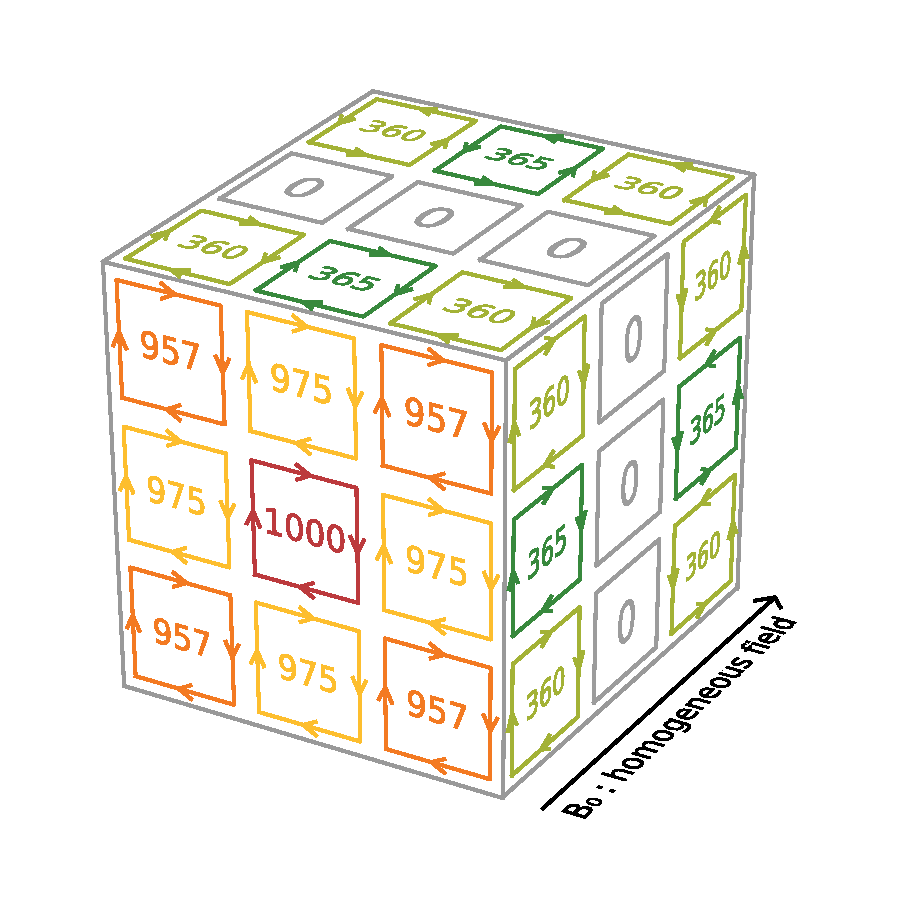
\includegraphics[width=\linewidth]{gfx/coils/homogeneous_tiles_norm_1000.pdf}
  \caption{A solution of a tile system with $N = 6 \times (3 \times 3)$ tiles on a unit cube for a homogeneous field. The volume of interest is a cube with side length 0.75, centered inside the unit cube. Numbers indicate currents in the tile coils in arbitrary units. The currents are normalized so that the highest is 1000. For clarity, the coils are depicted slightly smaller; in the model their edges overlap. The currents on the three invisible faces are by symmetry analogous to the visible ones.}
  \label{fig:homogeneous_tiles}
\end{figure}

% \begin{figure}
%   \centering
%   \includegraphics[width=0.8\linewidth]{homogeneous_performance.pdf}
%   \caption{Magnetic field produced by a coil designed for a homogeneous field (Fig.\,\ref{fig:homogeneous_tiles}). The grey lines depict the field lines. Contours show boundaries of 0.2, 0.5, 1 and 10\% magnitude deviation from an ideal homogeneous field. Horizontal section in the middle height is shown. The \emph{volume of interest} used in the optimisation has been depicted with a dashed line.}
%   \label{fig:homogeneous_performance}
% \end{figure}

\begin{figure*}[bth]
  \centering
  \subfloat{
    \label{fig:homogeneous_performance_a}
    \includegraphics[width=.45\linewidth]{gfx/coils/homogeneous_performance.pdf}}
  \quad
  \subfloat{
    \label{fig:homogeneous_performance_b}
    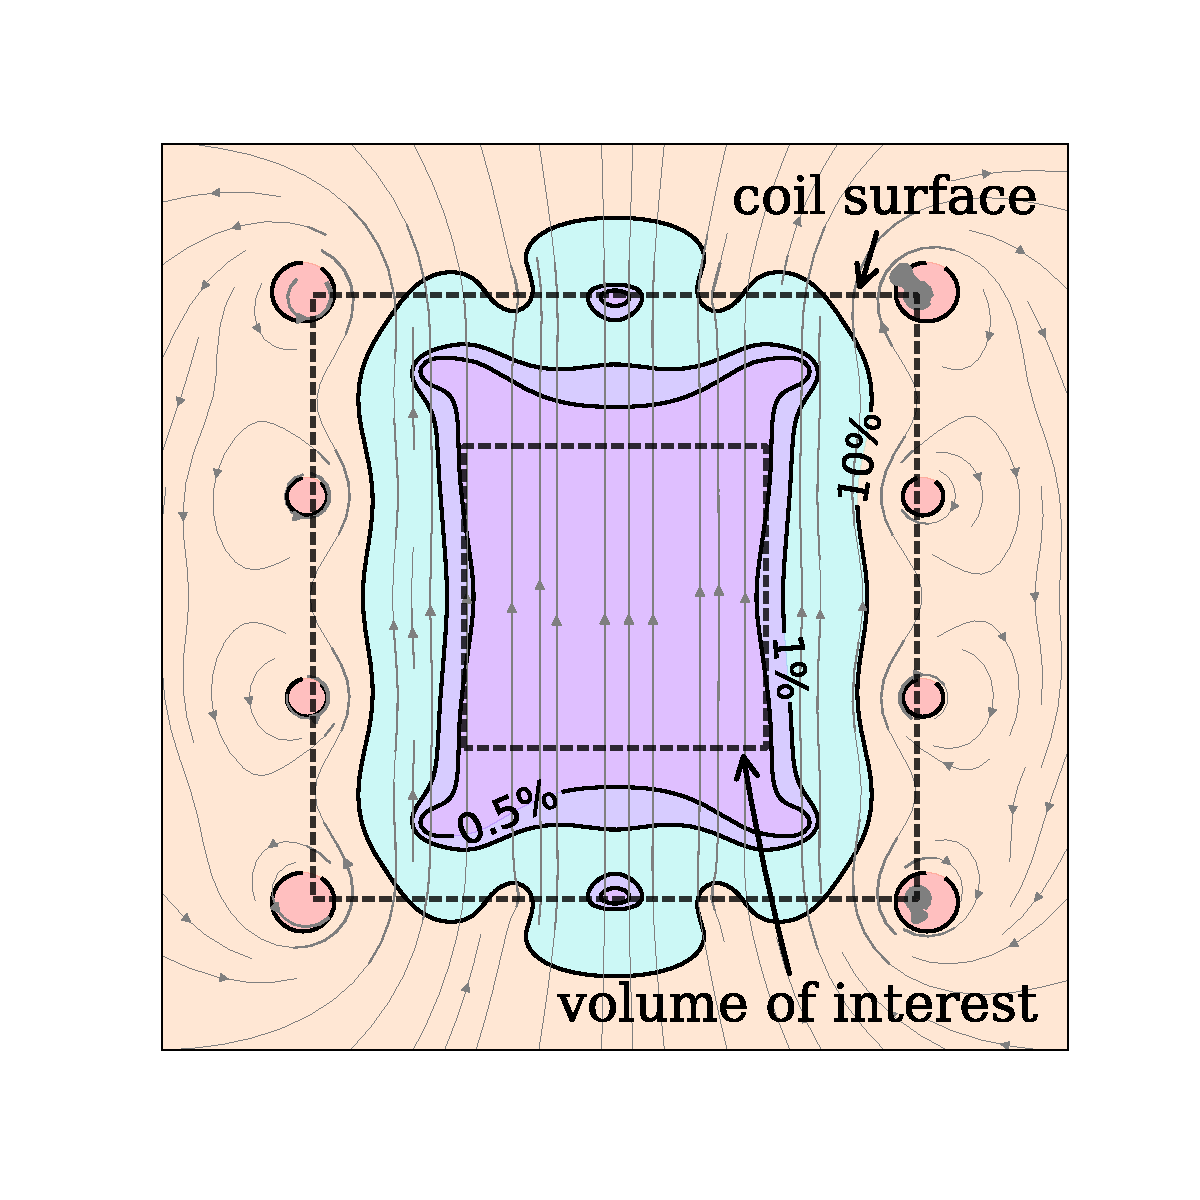
\includegraphics[width=.45\linewidth]{gfx/coils/homogeneous_performance_smaller_volume.pdf}}
  \caption{Magnetic field produced by a coil designed for a homogeneous field, with $N = 6 \times (3 \times 3)$ tiles on a unit cube. The field lines are depicted in grey. Contours show boundaries of 0.5, 1 and 10\% magnitude deviation from an ideal homogeneous field. Horizontal cross sections in the middle--height plane are shown. Two designs are presented. Left-hand side: the volume of interest is a cube with side length 0.75 (the individual tile coil currents are depicted in Fig.\,\ref{fig:homogeneous_tiles}), right-hand side: the size of volume of interest is reduced to 0.5.}
  \label{fig:homogeneous_performance}
\end{figure*}

Let us look at an example of a coil design on a unit cube with the number of tiles $N = 6 \times (3 \times 3)$ (see Fig.\,\ref{fig:homogeneous_tiles}). As the volume of interest we pick a cube, centered with the unit one, with side length 0.75 (with a regular mesh of $10 \times 10$ points on each face, a total of $m = 488$ points of interest). For the sake of simplicity we design a coil for a homogeneous field along an axis of the cube. The solution of Eq.\,\ref{eq:requirement}, $\mathbb{I}_0$, directly gives the currents in each tile, which are graphically depicted in Fig.\,\ref{fig:homogeneous_tiles}. Note that many currents almost cancel each other, in particular those along horizontal edges. The magnetic field produced by the solution is shown in Fig.\,\ref{fig:homogeneous_performance_a}, as a horizontal cut along the central plane. Contours show the relative deviation from the homogeneous field. Inside the volume of interest, depicted with a dashed line, the design goal of a homogeneous field, is reproduced with few per cent accuracy. The solution, and thus the contours too, depend on the choice of the volume of interest. In general, the smaller the volume of interest, the better the accuracy. If the side length of the volume of interest is decreased to 0.5, the accuracy improves to 1\%, as shown in Fig.\,\ref{fig:homogeneous_performance_b}. Note that the optimal solution, and thereby the shape of the precision contours, change. Naturally, one can increase the accuracy also by increasing the number of tiles.

% The tile system may find an interesting practical application. Once independently controllable tiles have been build, it can be used to produce an arbitrary field. The precision is only limited by the number of tiles.


\section{Simplification of the tile system}
The tile system may find an interesting practical application. Once independently controllable tiles have been built, it can be used to produce an arbitrary field. However, building many independently driven coils is a high price to pay if one wants to produce only a simple field. Additionally, note that each edge is shared between two tiles, and the effective current is the sum of two. They may add either constructively or destructively. If the given solution is dominated by subtraction of large currents, a lot of power is unnecessarily dissipated in the system. It turns out that both problems can be solved by simplifying the tile solution.

\begin{figure*}
  \centering
  % \subfloat[A coil designed for a homogeneous $50\,\mathrm{\micro T}$ field along the x--axis. A net current along each edge is shown.]{
  %   \label{fig:coils_homogeneous_3d}
  %   \includegraphics[width=.45\linewidth]{coil_homogeneous}}
  % \quad
  % \subfloat[XY section in the middle --- achieved relative compensation of the homogeneous field.]{
  %   \label{fig:coils_homogeneous_section}
  %   \includegraphics[width=.45\linewidth]{coil_homogeneous_section}}
  % \\
  \subfloat{
    \label{fig:coils_dipole_3d_1}
    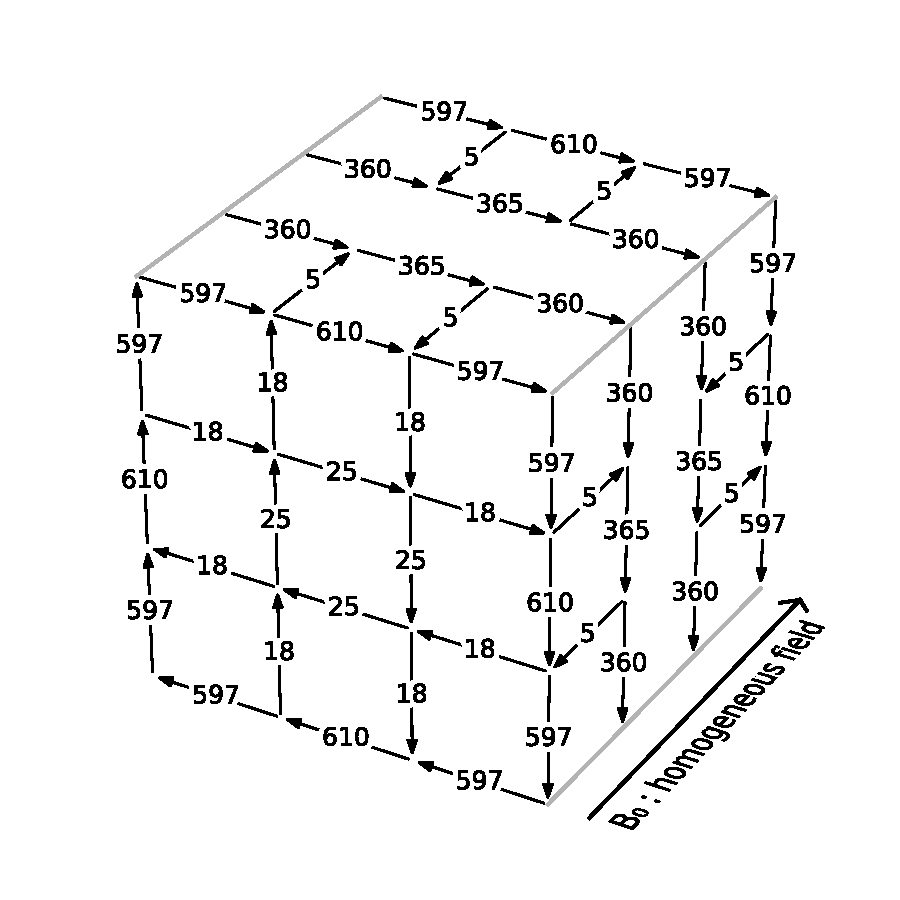
\includegraphics[width=.4\linewidth]{gfx/coils/algorithm_net_1.pdf}}
  \quad
  \subfloat{
    \label{fig:coils_dipole_section_0}
    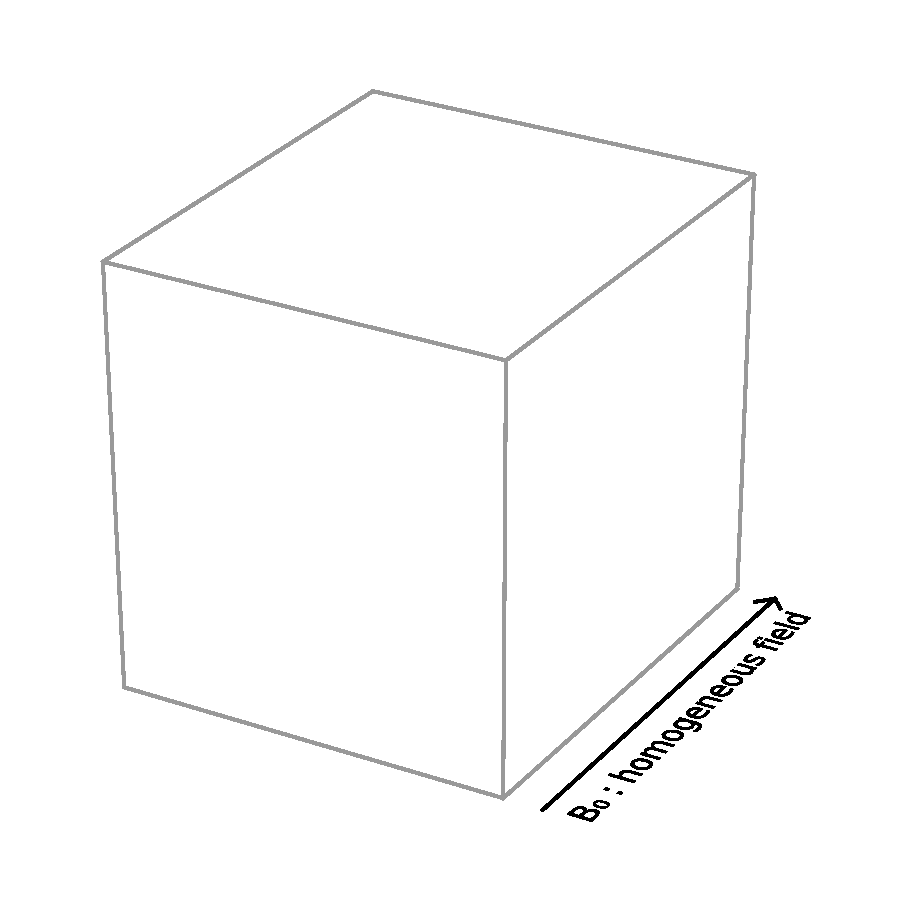
\includegraphics[width=.4\linewidth]{gfx/coils/algorithm_simplified_0.pdf}}
  \\
  \subfloat{
    \label{fig:coils_dipole_3d_3}
    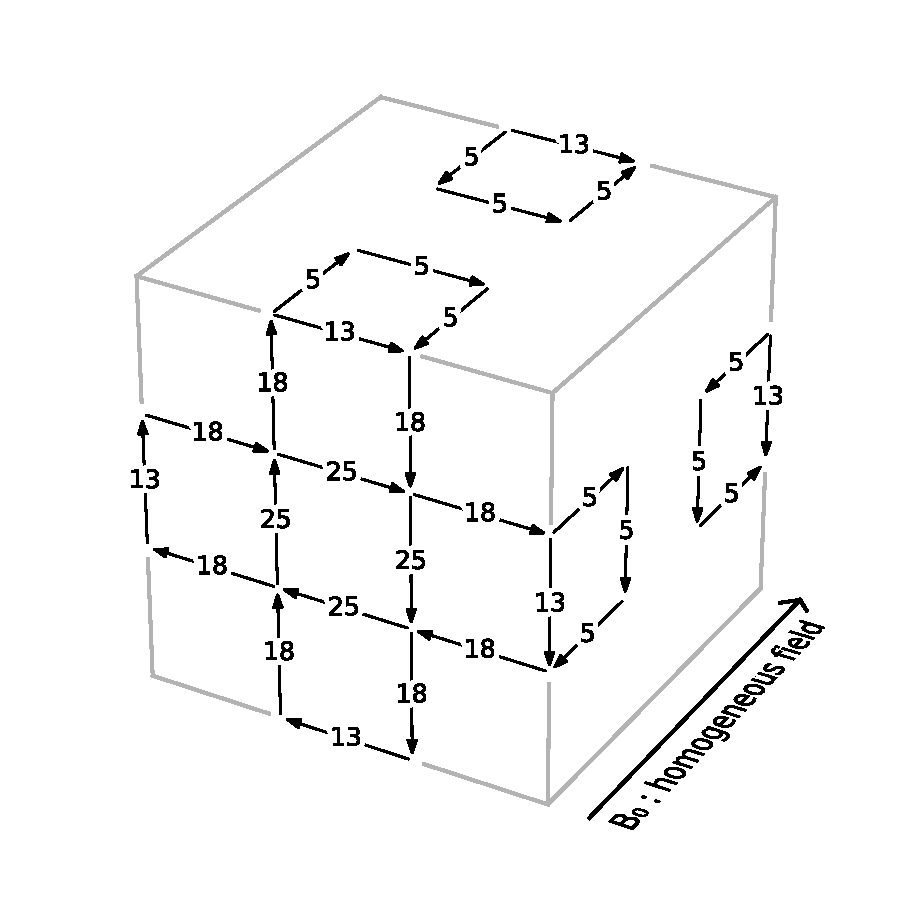
\includegraphics[width=.4\linewidth]{gfx/coils/algorithm_net_3.pdf}}
  \quad
  \subfloat{
    \label{fig:coils_dipole_section_2}
    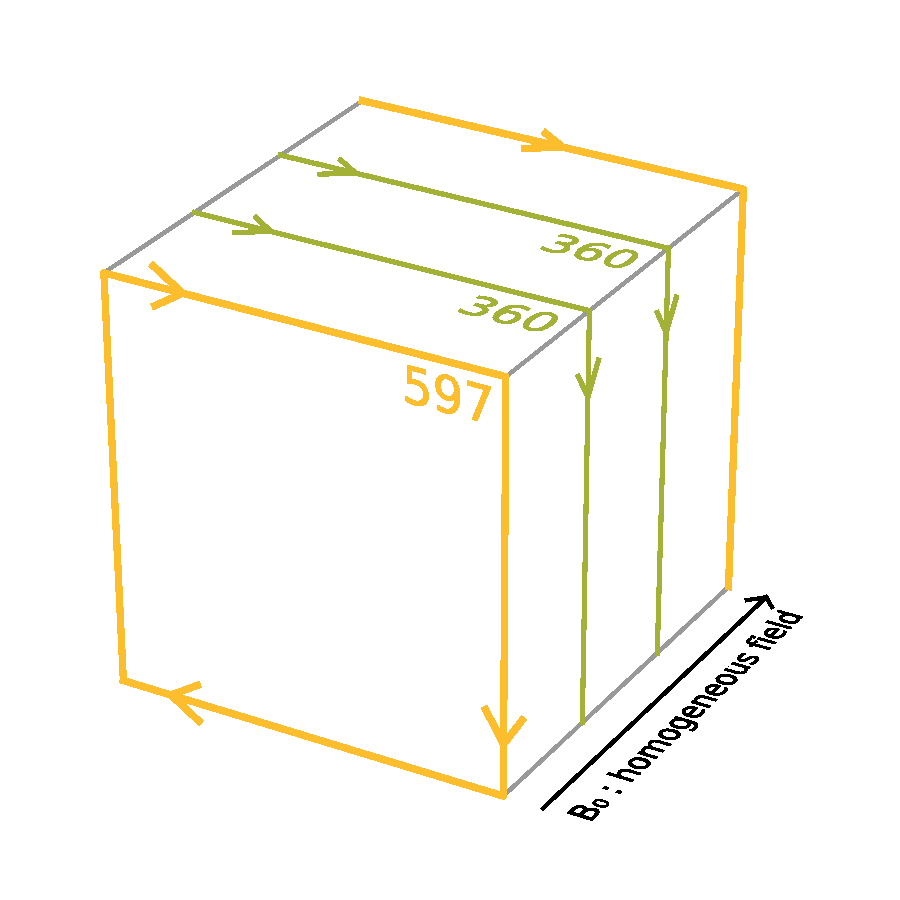
\includegraphics[width=.4\linewidth]{gfx/coils/algorithm_simplified_2.pdf}}
  \\
  \subfloat{
    \label{fig:coils_dipole_3d_5}
    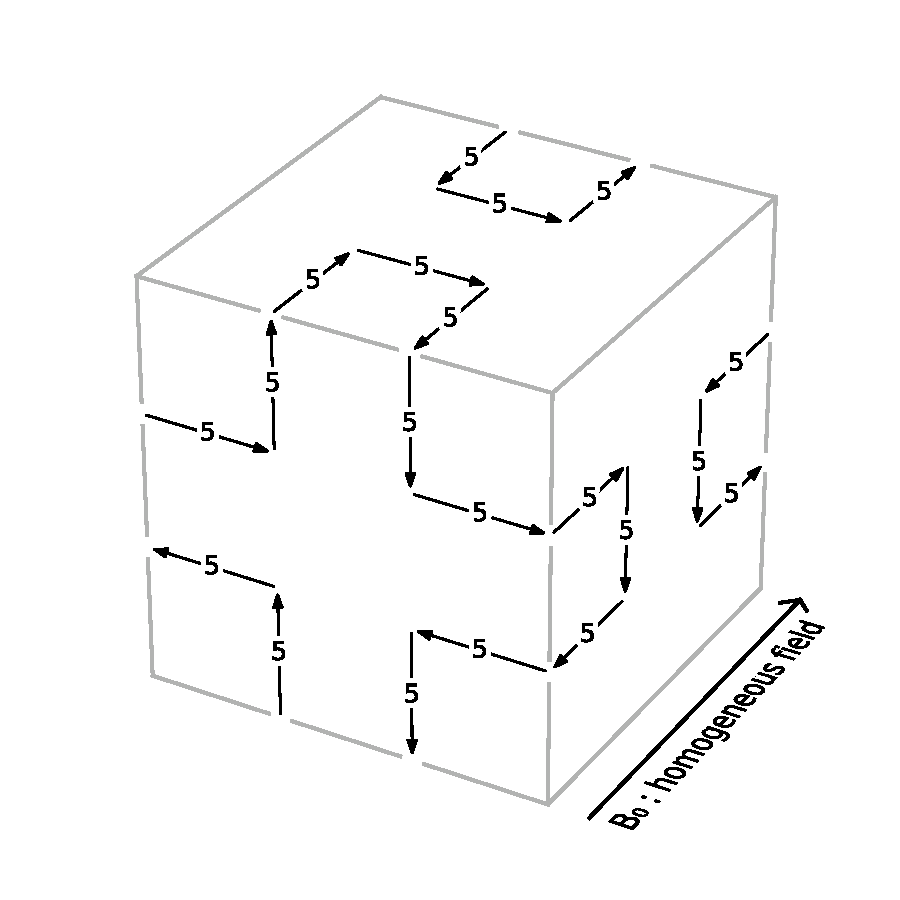
\includegraphics[width=.4\linewidth]{gfx/coils/algorithm_net_5.pdf}}
  \quad
  \subfloat{
    \label{fig:coils_dipole_section_4}
    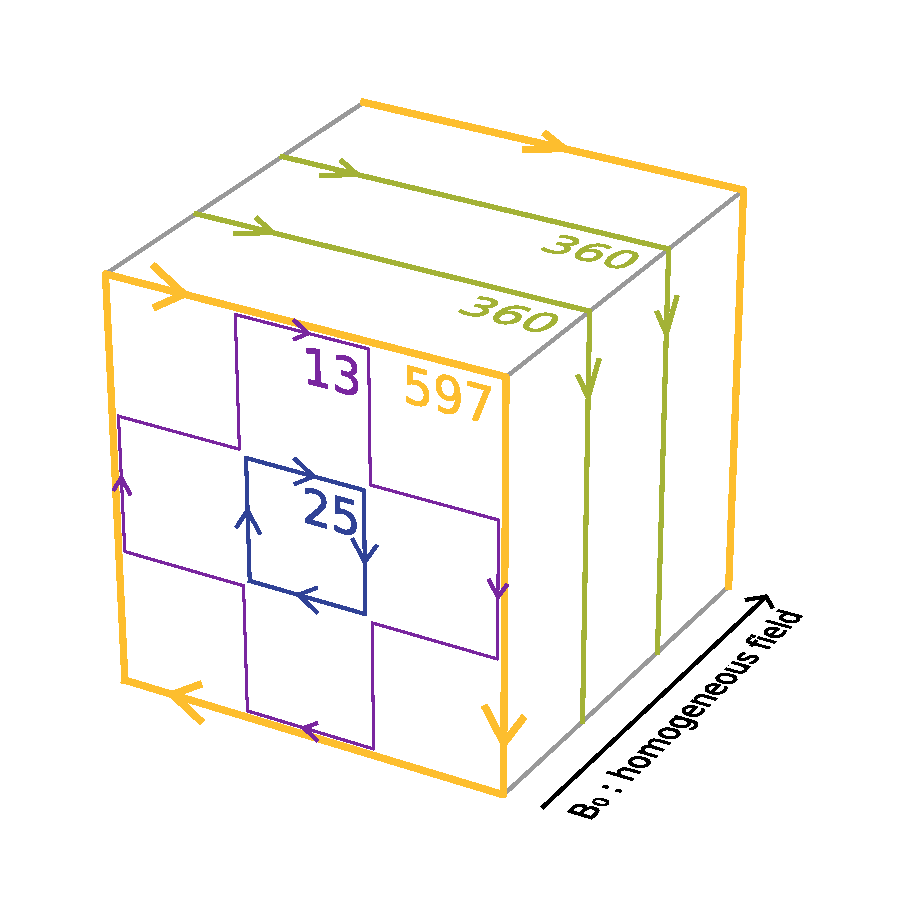
\includegraphics[width=.4\linewidth]{gfx/coils/algorithm_simplified_4.pdf}}
  \caption{Following the algorithm to simplify a coil. The left column shows the net of a current with the total current along edges of tiles. In each iteration the loop with the highest current is found and transferred onto the simplified solution, shown in the right column. We show iterations, from top: zeroth, fourth and eighth.}
  \label{fig:simplification_algorithm}
\end{figure*}

\begin{figure}
  \centering
  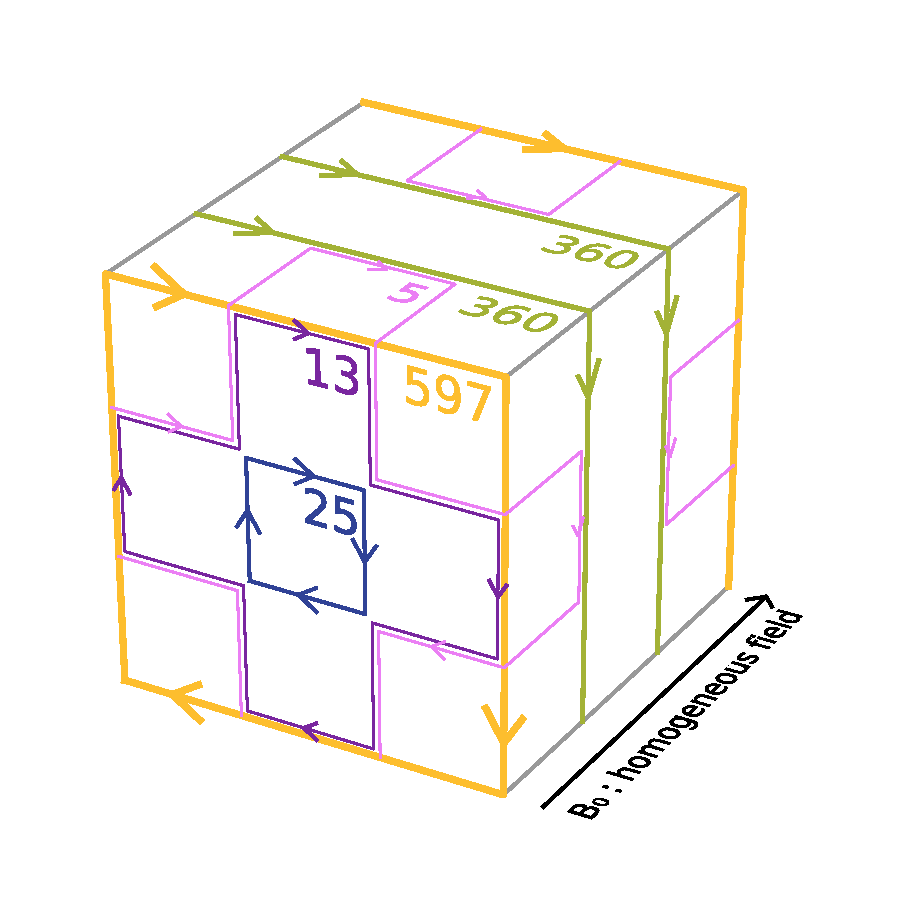
\includegraphics[width=\linewidth]{gfx/coils/algorithm_simplified_5.pdf}
  \caption{The coil designed for a homogeneous field, with $N = 6 \times (3 \times 3)$ tiles (Fig.\,\ref{fig:homogeneous_tiles}), simplified by adding the currents along each edge and decomposing into current loops.}
  \label{fig:homogeneous_coils}
\end{figure}

One starts by adding the currents of the adjacent tiles and assigning the sum to each common edge. The result is a complicated net of currents (upper left corner of Fig.\,\ref{fig:simplification_algorithm}). Still, each node fulfills Kirchhoff's laws. The net can then be decomposed into simple current loops by following the algorithm: Find in the net the loop with the highest current -- it will make the first one in the simplified solution. Then subtract from the net the current of the first loop along its edges. Continue to find the loop with the highest current in the modified net, which will give the second loop and continue. Some of the intermediate steps for the example (Fig.\,\ref{fig:homogeneous_tiles}) are shown in Fig.\,\ref{fig:simplification_algorithm}. The simplified solution is shown in Fig.\,\ref{fig:homogeneous_coils}. The currents in the simplified coil system are much smaller, the highest being 597 instead of 1000 and they always add constructively. Also the number of separate loops is decreased from 42 to 10. Still, the total current along each edge of a tile is exactly the same as in the tile configuration.

We conclude here our method of coil design. The simplified arrangement of coils is the optimal one, given the grid restriction, for approximating the magnetic field in the volume of interest. We continue to consider practical aspects, relevant for constructing the designs of our method.

% The simplified tile solution is what we consider a design of coil in our method. In the restricted space of coils with wires lying on the grid it is optimal for approximating the field $\mathbf{B}_0$ in the volume of interest.

% In practice, however, one may run into a problem.  Consider in particular an effective coil on the left-hand side of Fig.\,\ref{fig:uniform_field}, producing approximately a homogeneous field with a current of 2 in three loops.. The decomposition of this coil into a tile basis reveals that there is a current of 3 in eight tiles. In fact, the more fine the subdivision is, the more the currents in individual tiles increase above the highest effective current.
% \note{Don't show this one at all, but present the simplification of the homogeneous coil instead.}
% Figure\,\ref{fig:currents_blow_up} presets fragments of a side wall a coil with effectively current of 2 flowing along each edge downwards, for different number of tiles. Currents in individual tiles are written down. Already with each face divided into $4\times4$ tiles one needs cancelling currents of 5 and 3 only to produce an effective one of 2. There is, however, a way around this problem.

% \note{Maybe mention that when solving the Eq.\,\ref{eq:requirement} the problem of subtracting two large numbers exsists too, lowering the effective numerical resolution and, in extreme cases, rendering the problem unsolvable with a standard double precision numbers.}

% \begin{figure}
%   \centering
%   \includegraphics[width=0.8\linewidth]{uniform_field.pdf}
%   \caption{TODO}
%   \label{fig:uniform_field}
% \end{figure}
%
% \begin{figure}
%   \centering
%   \includegraphics[width=0.8\linewidth]{currents_blow_up.pdf}
%   \caption{TODO}
%   \label{fig:currents_blow_up}
% \end{figure}


% Firstly, in a coil constructed in the presented scheme often two currents effectively cancel. This happens whenever currents flow in opposite directions along a shared edge of adjacent base--coils.


\section{Practical considerations}
The primary practical advantage of our coil design method is that the coils are constrained to a predefined grid. This is contrary to other methods of coil design, where the position of the wires is the output of the procedure \cite{Turner1993, Beidler1990}. This may prove useful in applications with spatial constraints. Typically, coils need to be incorporated into a setup in which other components penetrate the surface on which the wires are laid. In our method it is possible to simply define the grid so that no collisions occur. Although the simple examples presented before used regular grids, we have not used symmetries to solve the problem. When many coils are designed and built, for instance to produce homogeneous magnetic fields in each of the three dimensions, they can all share the same grid. The grid can, for example, be constructed out of cable channels into which the wires are laid.

In our solution to produce the desired field one still needs a system of several coils, even in the simplified solution. The more complicated the goal field and the more tiles, the more different currents are needed across the individual loops, which quickly becomes impractical. There are several ways to tackle the problem.

The first way is to use only one current and adjust with the number of windings. In the example, when one decides for 60 as the maximum, then the current is $\mathrm{round}(597 / 60) = 10$. The 597, 360, 25, 13 and 5 would be created with 60, 36, 3, 1 and 1 windings respectively. A discretization error of $10 / 597 = 1.7\%$ is of the same order as the accuracy of the solution in representing the field (see Fig.\,\ref{fig:homogeneous_performance}). For more precise designs the numbers of windings get larger, which is troublesome to construct and causes the coils to have larger inductances.

% One decides on an elementary current and achieves different current ratios in loops by different numbers of windings. If we decide on an elementary current of 10, then the 597, 360, 25, 13 and 5 in our example would be created with 60, 36, 3, 1 and 1 windings respectively. A discretization error of $10 / 597 = 1.7\%$ is of the same order as the accuracy of the solution in representing the field (see Fig.\,\ref{fig:homogeneous_performance}). For more precise designs the numbers of windings get larger, which is troublesome to construct and causes the coils to have larger inductances.

A second way is to use a current divider. Connect the different loops in parallel, each with an appropriately chosen resistance in series. This way the ratios between the currents in each loop can be tuned precisely. However, a practical realization will most likely involve routing all loops out of the system where the current divider is installed. For more complicated coil systems with tens of different currents this may be impractical.

% A second way is to use a current divider. Connect the different loops in parallel, each with an appropriately chosen resistance in series. This way the ratios between the currents in each loop can be tuned precisely. However, under AC loads the impedances of the loops will increase, each according to its own inductance, thereby changing the current ratios. This will cause distortions in the produced field, the higher the frequency. Frequencies depend on the application, e.g. on the desired bandwidth of an actively stabilized feedback system. Additionally, the practical realization will most likely involve routing all loops out of the system where the current divider is installed. For more complicated coil systems with tens of different currents this may be impractical.

% Yet another way is to split the loops into decades of currents. In the coil we use as an example the currents $23.0,\ 13.8,\ 0.7,\ 0.2$ (in arbitrary units)
% may be constructed from a set of wires with three relative currents of 10, 1 and 0.1, in the following way:
% \begin{align*}
%   23.0 & = 2 \times 10 + 3 \times 1 + 0 \times 0.1 \\
%   13.8 & = 1 \times 10 + 3 \times 1 + 8 \times 0.1 \\
%   0.7 & = 0 \times 10 + 0 \times 1 + 7 \times 0.1 \\
%   0.2 & = 0 \times 10 + 0 \times 1 + 2 \times 0.1 \\
% \end{align*}
% In this way one can reach 1\% accuracy in reproducing the solution in practice with only 3 different currents to control, even for complicated designs. Those can be either split with a current divider if no good AC response is needed, or otherwise separately controlled.

Yet another way is to split the loops into decades of currents. In the coil we use as an example the currents 597, 360, 13, 7, 5 (in arbitrary units) may be constructed from a set of wires with three relative currents of 100, 10 and 1, in the following way:
\begin{align*}
  597 & = 5 \times 100 + 9 \times 10 + 7 \times 1 \\
  360 & = 3 \times 100 + 6 \times 10 + 0 \times 1 \\
  13 & = 0 \times 100 + 1 \times 10 + 3 \times 1 \\
  7 & = 0 \times 100 + 0 \times 10 + 7 \times 1 \\
  5 & = 0 \times 100 + 0 \times 10 + 5 \times 1 \\
\end{align*}
In this way one can reach better than 1\% accuracy in reproducing the solution in practice with only 3 different currents to control, even for complicated designs. Those can be either separately controlled or split with a current divider.

We do not consider any of the above ways superior. It is up to the particular application which is the best suited one.


% \note{Show: (a) a homogeneous field design on a 3x3x3 cube for simplicity and (b) a dipole field compensation on a 5x5x5 grid as showcase.}

% The simplest magnetic field is a homogeneous one. Figures\,\ref{fig:coils_homogeneous_3d} and \ref{fig:coils_homogeneous_section} show a coil designed for the homogeneous field. The \emph{coil surface} is a $\unit[1]{m^3}$ cube, the \emph{volume of interest} is a $\unit[0.75^3]{m^3}$ cube. The cube has been divided into $5 \times 5 \times 6 = 150$ tiles. The system achieves a 2\% homogeneity in the whole \emph{volume of interest}. Need to present also the wiring solution Fig.\,\ref{fig:coils_wiring}.

% The full power of this scheme is visible, when the desired $B_0$ field is complicated. One may want to counteract a fixed nearby dipole source. A coil designed for that is presented in Fig.\,\ref{fig:coils_dipole_3d}.


\section{An example of an application}
% The presented method may prove very useful to precision physics experiments. The measurement of the electric dipole moment, located in the Paul Scherrer Institute in Villigen, Switzerland, is one of the many experiments very sensitive to magnetic field. The measurement principle is spectroscopy of polarised neutrons in a combination of a magnetic and electric fields. Changes of the magnetic field directly disturb the measurement and may even induce a false signal. It is therefore crucial that the magnetic field is stable. At the same time the experiment, as it is typical, is located in an experimental hall, in direct vicinity of other setups. Many of the other experiments use strong magnets, often ramped up and down daily.

% The measurement of the electric dipole moment of the neutron, located in the Paul Scherrer Institute in Villigen, Switzerland, is very sensitive to the magnetic field. The measurement is based on a spectroscopy of neutrons. Details can be found in \note{cite}.

% The electric dipole moment of the neutron is an observable that directly links to fundamental CP symmetry breaking. I

The presented method may prove useful to precision physics experiments. Among them is the measurement of the electric dipole moment of the neutron, an observable providing direct insight into the fundamental $\mathcal{CP}$ symmetry breaking in the strong interaction \cite{khriplovic:1997}. In the experiment at the Paul Scherrer Institute the electric dipole moment of the neutron is measured with a precise spectroscopy of polarized neutrons in a combination of electric and magnetic fields \cite{Baker2011}. The precision of the measurement sets very strict requirements for the magnetic field stability, yet the experiment is only one of the many in the experimental hall. Some of the other setups use strong magnets, often ramped up and down daily. The neutron electric dipole moment measurement would not be possible without counter measures against the external magnetic field changes.

The experiment uses an active magnetic field stabilization system. The apparatus is located in the middle of a set of large coils, connected in a feedback loop with magnetic field sensors. The present system is described in detail in \cite{Afach2014}. The geometry of the coils, six in total, is very simple: each coil is a rectangle and they are all arranged in three perpendicular Helmholtz--like pairs. The simple geometry causes the volume in which the field is stabilized (the volume of interest) to be small relative to the size of the coils. Only thanks to the sufficient space around the less than 3$\,$m large apparatus it was possible to make these simple coils large enough, 6--8$\,$ meters side length, for the experiment to fit in the volume of interest. Also, the variety of field shapes that can be compensated is limited to homogeneous ones (parallel currents in a Helmholtz--like pair) plus fields created when each coil is controlled separately.

Using the method presented here to design the active compensation coils offers improvements in two areas. Firstly, the size of the coils could be decreased, or the size of the experimental set-up increased, without loss of performance. Secondly, more coils could be built, extending the range of possible fields to be compensated. These could either be generic: e.g. pure independent gradients, or coils dedicated to counteract a particular known disturbance, designed based on a field map as the goal field in the described method.


% One needs not to worry about possible spacial conflicts, as the method guarantees that all the coils are constrained to the grid on which they are designed.


\begin{figure*}
  \centering
  % \subfloat[A coil designed for a homogeneous $50\,\mathrm{\micro T}$ field along the x--axis. A net current along each edge is shown.]{
  %   \label{fig:coils_homogeneous_3d}
  %   \includegraphics[width=.45\linewidth]{coil_homogeneous}}
  % \quad
  % \subfloat[XY section in the middle --- achieved relative compensation of the homogeneous field.]{
  %   \label{fig:coils_homogeneous_section}
  %   \includegraphics[width=.45\linewidth]{coil_homogeneous_section}}
  % \\
  \subfloat{
    \label{fig:coils_dipole_3d}
    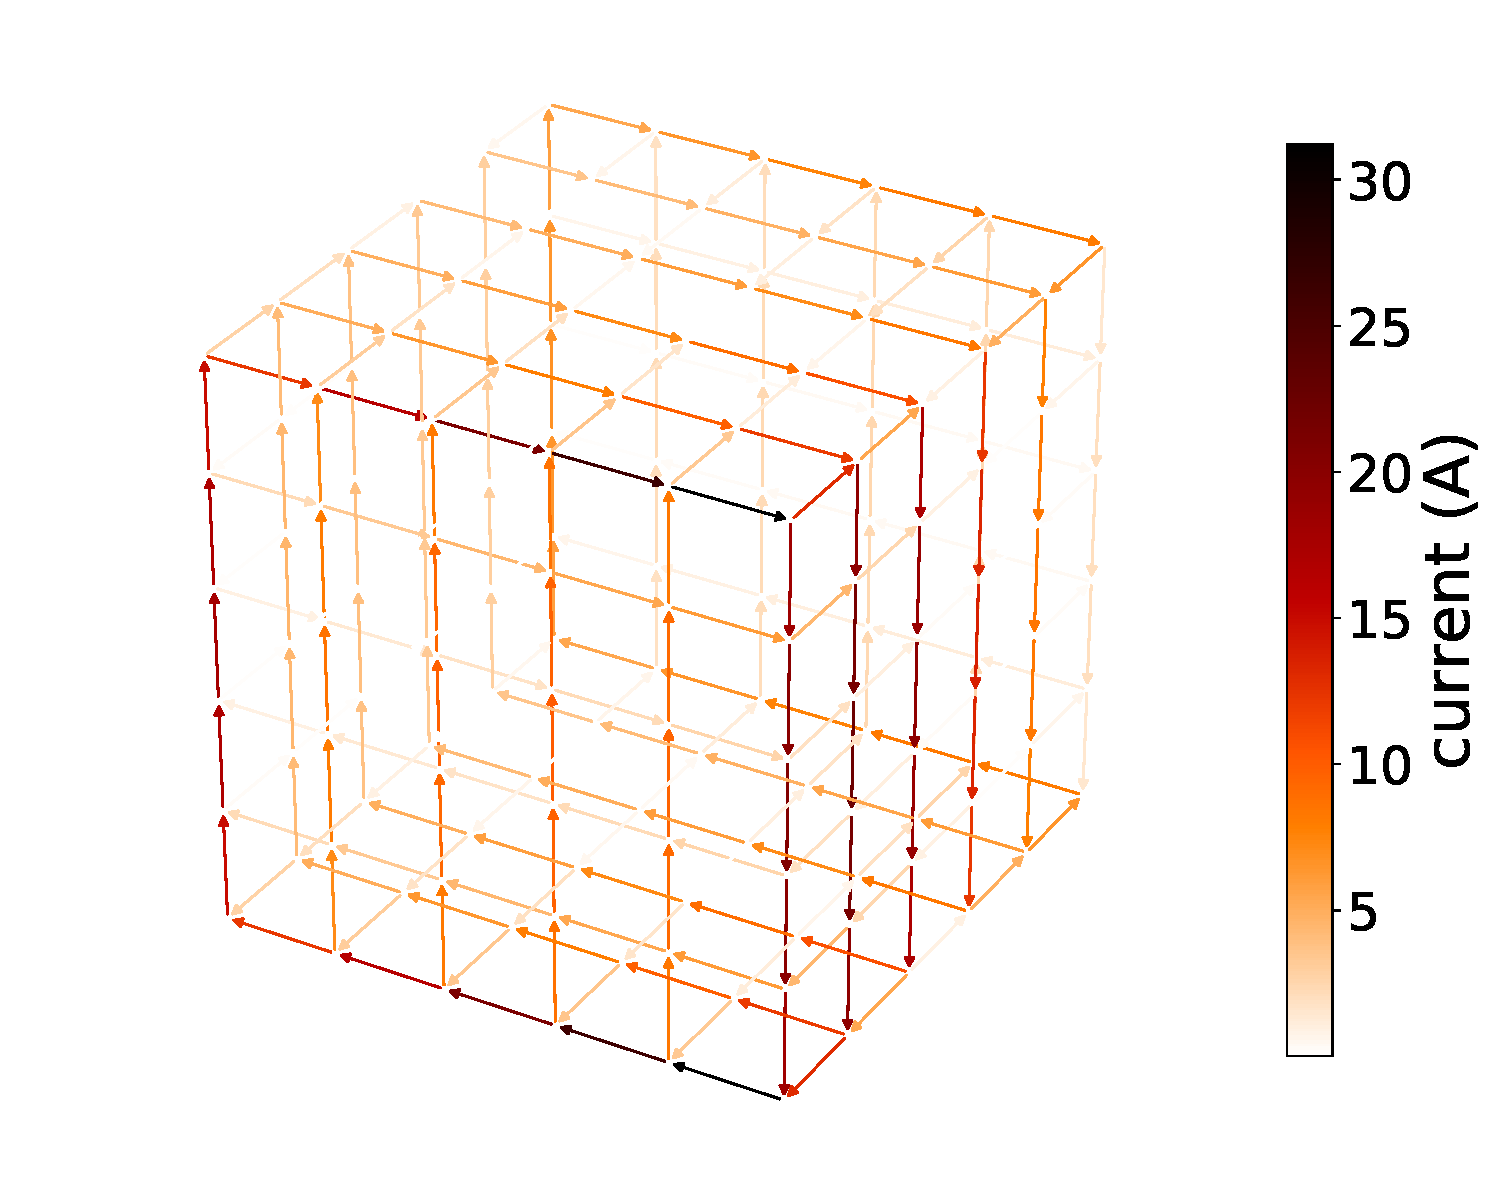
\includegraphics[width=.35\linewidth]{gfx/coils/coil_dipole.pdf}}
  \quad
  \subfloat{
    \label{fig:coils_dipole_section}
    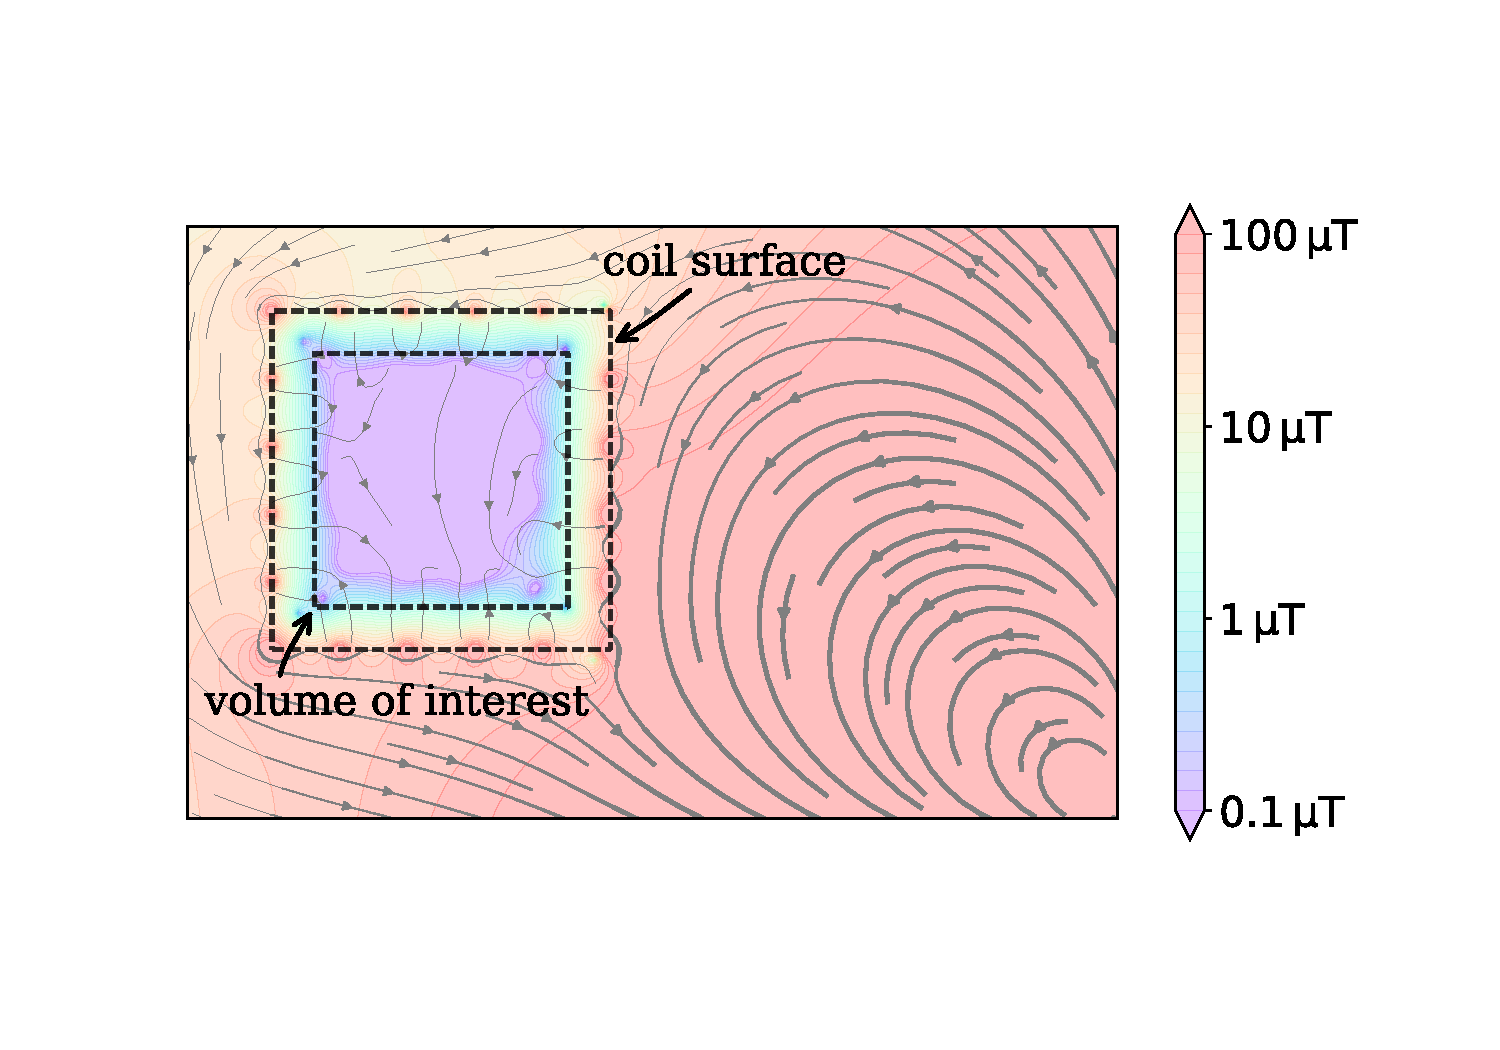
\includegraphics[width=.55\linewidth]{gfx/coils/coil_dipole_section_with_dipole.pdf}}
  \caption{A coil designed on a unit cube with $5 \times 5$ tiles per face to shield against a dipole disturbance. The dipole is located, relative to the center of the unit cube, two units to the right and one unit to the front. It is located in the middle height of the cube. The volume of interest has a side length of 0.75. On the left--hand side the total current along each edge of the dipole compensation coil is depicted. On the right--hand side the magnetic field is shown. The magnetic field lines are shown in grey, the volume of interest and the coil surface with dashed lines. The colors depict the magnitude of the magnetic field (capped at 0.1 and 100\,µT). A horizontal cross section in the middle height is shown. The dipole source is located in the lower right corner of the plot and points parallel to the plane of the plot. The magnitude of the field in the volume of interest is reduced from tens of microteslas down to below one.}
  \label{fig:showcase}
\end{figure*}





% Let us consider a problem that may occur for an experimental physicist. He is conducting a high-precision experiment, sensitive to magnetic fields. The experiment is located in an experimental hall among tens of others. It so happens, that his neighbour uses a very strong magnet, whose stay field totally destroys the precise experiment. The experimentalist knows exactly the shape of the stray field produced by the magnet from the specifications. He knows, that he can use this information to design a compensation coil around his apparatus. Not only our method will give the physicist the solution, no matter how complicated the stray field looks like. He can even carefully define a grid which goes around all the mechanical constraints of his apparatus and the experimental hall. In figure~\ref{fig:showcase} we present what a coil designed in a situation like that might look like.



% \begin{figure}[bth]
%   \centering
%   \includegraphics[width=.6\linewidth]{wiring}
%   \caption
%   [TODO]
%   {The wiring solution. \note{Present a full picture of a 3x3 design for a homogeneous field.}}
%   \label{fig:coils_wiring}
% \end{figure}


% \section{A good set of coils for an arbitrary field}
% \note{Need to cite \cite{Turner1993}}
%
% When one wants to be able to produce an arbitrary field, it is best to use an orthogonal expansion, in analogy to the Taylor expansion for functions. Furthermore, it is desired that the terms of the expansions are natural for the system considered (as spherical harmonics used to describe the wavefunctions of electrons in atomic systems are solutions to the Schrödinger equation themselves). Also, from the point of view of control, it is much easier to control an orthogonal system. See eg. \,\citep{Branch1984} for detailed motivation (really?). In an expansion one can gradually improve the system.
%
% Such an expansion exists: \emph{carthesian harmonic polynomials}.
% \begin{equation}
%   \mathbf{B}(\mathbf{r}) = \sum_{n}\,H_n\mathbf{P}_n(\mathbf{r})
% \end{equation}
% where $H_n$ are the expansion coefficients. They satisfy Maxwell's equations, so it is always theoretically possible to create a coil that produces the eigenfunctions. The table~\ref{tab:coils_carthesian_harmonics} presents first few of them.
%
% \begin{table}
%   \centering
%   \begin{tabular}{c|ccc}
%     n & $P_n^x(\mathbf{r})$ & $P_n^y(\mathbf{r})$ & $P_n^y(\mathbf{r})$ \\ \hline
%     1 & 1 & 0 & 0 \\
%     2 & 0 & 1 & 0 \\
%     3 & 0 & 0 & 1 \\ \hline
%     4 & $x$ &  0  & $-z$ \\
%     5 & $y$ & $x$ &   0  \\
%     6 &  0  & $y$ & $-z$ \\
%     7 & $z$ &  0  & $ x$ \\
%     8 &  0  & $z$ & $-y$ \\
%   \end{tabular}
%   \caption{Carthesian harmonic polynomials.}
%   \label{tab:coils_carthesian_harmonics}
% \end{table}
%
% The first three terms are homogeneous fields. Further five are the five independent gradients.


\section{Conclusion}
Coil design is a complicated and very technical problem, especially when high accuracy is required. We presented a method that is simple in terms of both underlying math and computational effort. We believe that the design method can find its niche in practical applications, where spatial constraints play a significant role and a percent level in accuracy of the produced field is acceptable.

For the sake of clarity we explained the method on a simple example. We designed a coil for a homogeneous field with only few tiles. However, the method is much more powerful. We conclude by presenting, in Fig.\,\ref{fig:showcase}, a showcase design with $N = 6 \times (5 \times 5) = 150$ tiles for compensating a nearby dipole source.

We publish the software implementation of the coil design, including examples, as open--source \cite{Coilsjlcode}.

We would like to thank Georg Bison, Allard Schnabel and other members of the nEDM at PSI collaboration for fruitful discussions. This work was supported by the Swiss National Science Foundation under grant 200020\_162574.







%%%%%%%%%%%%%%%%%%%%%%%%%%%%%%%%%%%%%%%%%%%%%%%%%%%%%%%%%%%%%%%%%%%%%%%%%%
%%%%% END PASTED PUBLICATION %%%%%%%%%%%%%%%%%%%%%%%%%
%%%%%%%%%%%%%%%%%%%%%%%%%%%%%%%%%%%%%%%%%%%%%%%%%%%%%%%




\section{Introduction}

Motivation... Where the problem is encountered. Need some citations here.

Coils producing a magnetic field of desired spatial distribution are a necessary ingredient in many engineering and physics applications.

In active magnetic field stabilisation systems the desired field shape is not even known beforehand -- a system capable of producing a aoeu is desired.
The need for coils producing magnetic fields of a desired spatial distribution has
Elaborate methods have been developed, mostly focusing on precision of created field.
Extensive literature to design sophisticated coils.
See an overview by \citeauthor{Turner1993} \citep{Turner1993}.

In particular finds use in active magnetic field stabilisation systems, eg. in nEDM experiments or in PTB (really?).

An interesting approach to coil design was presented by \citeauthor{Compton1982} \citep{Compton1982}. He proposed to divide a surface into small elements and solve for current density in each element. This is very general and powerful idea, albeit the solution is likely to be hard to build.

Most of modern coil design approaches focus on increasing the precision of the created field, giving designs that are very difficult to manufacture. The presented approach focuses on versatility and ease of practical realisation, which makes it potentially useful for large scale builds and systems employing multiple coils.

Mention the main feature of this approach --- the spatial constraint on the location of the wires? Needs some explanation probably.

We begin by presenting a method to describe a subset of all possible coils that can be built on a surface on a square. Next we show how this can be used on a cube to describe coils around a volume. With this algebraic language the coil design is simplified to solving one linear least--squares problem.


\section{Model}
\subsection{Coils as a linear space}
Consider all possible coils that can be constructed by laying wires on a surface of a square. The possibilities are as endless as they are hard to grasp mathematically. What is presented is a language that makes this problem suprisingly simple.

Coils can be seen an vectors in a linear space. One coil spans a one--dimensional space of magnetic fields it can produce. Adding a second coil creates a system spanning a two--dimensional space of fields, thanks to the magnetic field being additive. Four square coils tiled to form a larger square form a four--dimensional space, which is a subset of coils possible to construct on the larger square's surface. This size of the subset we restrict ourselves to is controlled by $N$ --- the number of \emph{base coils} forming the grid. Any coil, member of the subset, is fully described by a vector of $N$ relative currents in each of the \emph{base coils} --- denoted by $\mathbb{I}$. The problem of coil design is thereby simplified to finding a vector $\mathbb{I}$ in a linear space.
% The four coils form a complete linear basis of coils on the surface for any coils that have wires going only along the edges --- see Fig.\,\ref{fig:coils_tile_basis}. This is a very convenient subspace of all coils possible to build on a square. The possible to realise subspace may be enlarged by refining the division into tiles. But as a coil is equivalent to the field it produces, one can just as well say that they form a four--dimensional \emph{space of coils}.

\begin{figure}[bth]
  \myfloatalign
  \subfloat[A basis of four base--coils on a surface. Three vectors are presented together with their explicit coordinates in the basis.]
  {\label{fig:coils_tile_basis}
  \includegraphics[width=.45\linewidth]{gfx/tile_basis}}
  \quad
  \subfloat[A coil which spans one--dimensional subspace of coil--vectors on a cuboid that produces no magnetic field.]
  {\label{fig:coils_tile_kernel}
  \includegraphics[width=.45\linewidth]{gfx/tile_kernel}}
  \caption{Coils as a vector space.}
\end{figure}

A cube consists of six square faces. Therefore the set of \emph{base coils} can be constructed by dividing each face into a grid. However, for a set of $N$ grid coils the space of fields possible to produce has dimension $N-1$. Consider six square coils combined into a cube form only a five--dimensional space of coils, as same current flowing in each of the coils produces no field, as explained in Fig.\,\ref{fig:coils_tile_kernel}. Dividing the faces of the cube into $N$ tiles provides a simple basis for many coils that can be built around a volume.

% A cube consists of six square faces. On each a grid may be constructed, forming a set of $N$ \emph{base coils}.  smaller The problem of coil design is much simpler, as now it is a problem in a finite--, $N$--dimensional linear space. A $coil$ is fully described by a set of $N$ currents in each of the \emph{base coils} --- $\mathbb{I}$. At the cost of restraining oneself to coils that can have wires only along the edges of the tiles, one gains a tremendous simplification of the problem.
% However, six square coils combined into a cube form only a five--dimensional space of coils, as same current flowing in each of the coils produces no field, as explained in Fig.\,\ref{fig:coils_tile_kernel}. Dividing the faces of the cube into $N$ tiles provides a simple basis for many coils that can be built around a volume.

The mechanical constrain can be of tremendous advantage. Every coil in this subspace is guaranteed to be mechanically constrained to the edges of the tiles. Once a mechanical support is build, coil may be designed and added even later.

In a coil constructed in the presented scheme in general a lot of currents, flowing in an opposite direction along the same edge, would cancel. For each edge there are two adjacent \emph{base coils}, so inevitably some currents will, at least partially, cancel. A coil can always be simplified by simply adding the two currents flowing along each edge, as it is presented in Fig.\,\ref{fig:coils_tile_basis}.


\subsection{Coil design}
In the problem of coil design one wants to create \emph{a coil that will best approximate a given field in a certain volume}. Let us call this volume \emph{the volume of interest}. It can be of an arbitrary shape and is located fully inside the coil system (the cube). One can pick an ensemble of $n$ points on the surface of the \emph{volume of interest} (its surface is sufficient because $\nabla \mathbf{B} = 0$). Let us denote the combined vector, dimension $3n$, of magnetic field in each of the point by $\mathbb{B}$.

% Note, that magnetic field produced by a coil at a given point in space is proportional to the current in this coil. For a fixed direction in a fixed point in space it is a linear combination of currents of all coils in the system. Now, if we consider a vector of 3 spatial directions in $M$ points \ie, dimension $3M$. It can be obtained from an arbitrary coil $C$ by multiplying it by a $NNN \times 3M$ matrix $\mathbb{M}$. This matrix encodes the geometry of the system and may be pre-calculated.

Note, that magnetic field produced by a coil at a given point in space is proportional to the current in this coil. For a fixed direction in a fixed point in space it is a linear combination of currents of all coils in the system. In an absence of external magnetic field the system is thus described by a simple linear equation:
\begin{equation}
  \mathbb{B} = \mathbb{M} \, \mathbb{I}
\end{equation}
where $\mathbb{M}$ is a $3n \times N$ matrix encoding the geometry of the system.

For rectangular tiles the matrix can be easily calculated using the formula given by \citeauthor{Reta-Hernandez1998}~\citep{Reta-Hernandez1998}). If the tiles are not rectangular then it can still be analytically obtained by integration of the Biot--Savart law.

The goal is to design a coil that would best approximate a field $\mathbf{B}_0$ in the \emph{volume of interest}. In the $n$ points of interest the field has values $\mathbb{B}_0$ --- a vector similar to $\mathbb{B}$. The \emph{coil} is evaluated by solving the following linear problem for $\mathbb{I}$:
\begin{equation}
  \mathbb{M} \, \mathbb{I} \stackrel{!}{=} \mathbb{B}_0
\end{equation}
If one picks enough points that $\mathrm{dim}(\mathbb{B}) > \mathrm{dim}(I)$, then the equation is an over--determined set of linear equations. The solution is found by the ordinary least--squares method.

Solving the least--squares problem will produce for \emph{any} field $\mathbf{B}_0$
\emph{the} optimal coil in the restricted space. I emphasise, that the spatial restriction is
may be highly desirable. Especially if a number of coils, each producing different field, is to be would around the volume. In the presented scheme adding a new coil will not cover the \emph{surface of the coils} more densely, as opposed to other schemes in the literature.

\subsection{Examples}
The simplest magnetic field is a homogeneous one. Figures\,\ref{fig:coils_homogeneous_3d} and \ref{fig:coils_homogeneous_section} show a coil designed for the homogeneous field. The \emph{coil surface} is a $\unit[1]{m^3}$ cube, the \emph{volume of interest} is a $\unit[0.75^3]{m^3}$ cube. The cube has been divided into $5 \times 5 \times 6 = 150$ tiles. The system achieves a 2\% homogeneity in the whole \emph{volume of interest}.

The full power of this scheme is visible, when the desired $B_0$ field is complicated. One may want to counteract a fixed nearby dipole source. A coil designed for that is presented in Fig.\,\ref{fig:coils_dipole_3d}.

\begin{figure}[bth]
  \myfloatalign
  \subfloat[A coil designed for a homogeneous $50\,\mathrm{\micro T}$ field along the x--axis. A net current along each edge is shown.]{
    \label{fig:coils_homogeneous_3d}
    \includegraphics[width=.45\linewidth]{gfx/coil_homogeneous}}
  \quad
  \subfloat[XY section in the middle --- achieved relative compensation of the homogeneous field.]{
    \label{fig:coils_homogeneous_section}
    \includegraphics[width=.45\linewidth]{gfx/coil_homogeneous_section}}
  \\
  \subfloat[A coil designed for a dipole disturbance, $3\,\mathrm{kNm/T}$, $2.2\,\mathrm{m}$ away from the centre with 5x5 base tiles per face.]{
    \label{fig:coils_dipole_3d}
    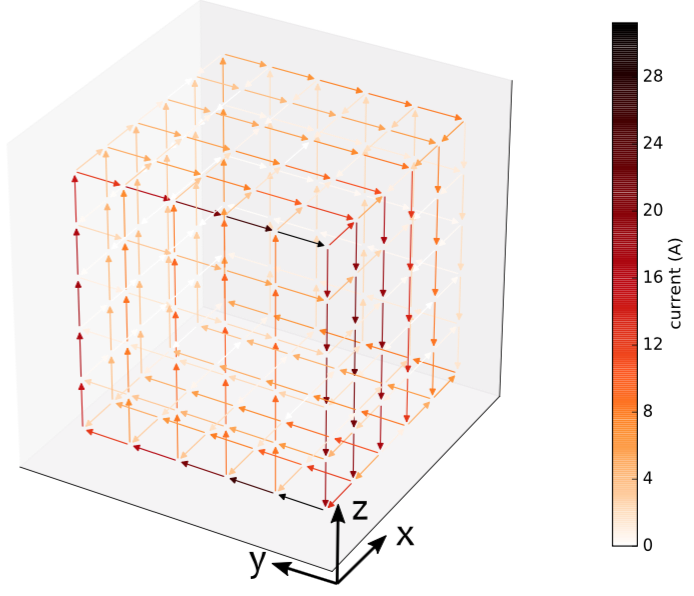
\includegraphics[width=.45\linewidth]{gfx/coil_dipole}}
  \quad
  \subfloat[XY section in the middle --- achieved relative compensation of the homogeneous field.]{
    \label{fig:coils_dipole_section}
    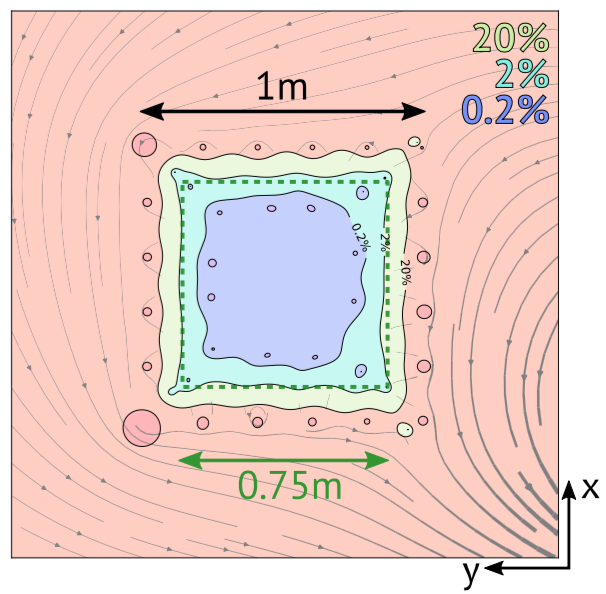
\includegraphics[width=.45\linewidth]{gfx/coil_dipole_section}}
  \caption{Coils as a vector space.}
\end{figure}


\section{A good set of coils for an arbitrary field}
When one wants to be able to produce an arbitrary field, it is best to use an orthogonal expansion, in analogy to the Taylor expansion for functions. Furthermore, it is desired that the terms of the expansions are natural for the system considered (as spherical harmonics used to describe the wavefunctions of electrons in atomic systems are solutions to the Schrödinger equation themselves). Also, from the point of view of control, it is much easier to control an orthogonal system. See eg. \,\citep{Branch1984} for detailed motivation (really?). In an expansion one can gradually improve the system.

Such an expansion exists: \emph{carthesian harmonic polynomials}.
\begin{equation}
  \mathbf{B}(\mathbf{r}) = \sum_{n}\,H_n\mathbf{P}_n(\mathbf{r})
\end{equation}
where $H_n$ are the expansion coefficients. They satisfy Maxwell's equations, so it is always theoretically possible to create a coil that produces the eigenfunctions. The table~\ref{tab:coils_carthesian_harmonics} presents first few of them.

\begin{table}
  \centering
  \begin{tabular}{c|ccc}
    n & $P_n^x(\mathbf{r})$ & $P_n^y(\mathbf{r})$ & $P_n^y(\mathbf{r})$ \\ \hline
    1 & 1 & 0 & 0 \\
    2 & 0 & 1 & 0 \\
    3 & 0 & 0 & 1 \\ \hline
    4 & $x$ &  0  & $-z$ \\
    5 & $y$ & $x$ &   0  \\
    6 &  0  & $y$ & $-z$ \\
    7 & $z$ &  0  & $ x$ \\
    8 &  0  & $z$ & $-y$ \\
  \end{tabular}
  \caption{Carthesian harmonic polynomials.}
  \label{tab:coils_carthesian_harmonics}
\end{table}

The first three terms are homogeneous fields. Further five are the five independent gradients.


\section{Construction}
The first step is to define the \emph{coil surface}. Afterwards the surface has to be divided into tiles. The tiles need not necessarily be squared. They may not be rectangular, on even not flat. The finer the division, the better the field can be approximated, but also the harder it is to construct the system. A simple choice is to choose the coil surface to be a cuboid and the tiles to be rectangles.


Exploit symmetries --- a homogeneous coil may be viewed a sum of a number of
much simpler to construct coils, which are then connected in series.

\begin{figure}[bth]
  \myfloatalign
  \includegraphics[width=.6\linewidth]{gfx/coils/wiring}
  \caption
  [TODO]
  {%FIXME directly copied from the SFC paper
The wiring solution.}
  \label{fig:coils_wiring}
\end{figure}

Each edge can have any real current (albeit the Kirchoff law is fulfilled).
However, to keep the number of control channels reasonably small, they need
to be driven with one current source. Two techniques may be used:
\begin{enumerate}
  \item using a different number of wires, connected in series --- only discrete
  \item varying resistance of different parts of the coil connected in parallel
  --- can be adjusted continuously, but causes power dissipation.
\end{enumerate}

1A, 0.1A, 0.001A wires solution --- keeps the number of windings reasonably small.
With a simple use of additional resistors each coil may be still driven with only
one power supply --- \emph{provide a figure}.

\begin{figure}[bth]
  \myfloatalign
  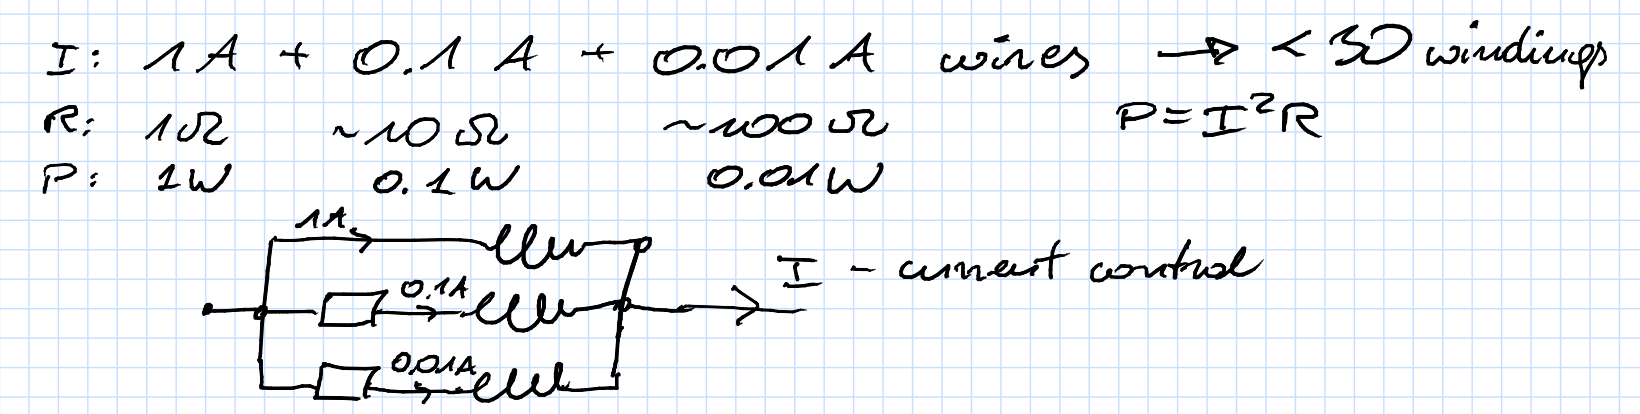
\includegraphics[width=.6\linewidth]{gfx/coils/current_discretisation}
  \caption
  [TODO]
  {%FIXME directly copied from the SFC paper
The wirining solution.}
  \label{fig:coils_current_discretisation}
\end{figure}

Care has to be taken to balance voltage and current needs for the power supplies.

Parameters to vary: number of windings, thickness of cable (price). Note also
the inductance of the coils.

\subsection{Possible generalisations}
\begin{enumerate}
  \item the surface does not need to be cubic
  \item
\end{enumerate}



\section{Practical application --- SFC system}
\subsection{Surrounding Field Compensation in the nEDM experiment}
The main challenge of the nEDM experiment is reaching a magnetic field stability on the picotesla level on a timescale of minutes. At the same time the experiment is set up in a research facility, where strong magnets are common. In fact, at the experimental site the compass points in different directions throughout the day.

The main part of attenuation of the magnetic field is done by four layers of \mbox{μ-metal} --- material with very high permeability (around 400\,000). However, \mbox{μ-metal}, being a ferromagnetic, is itself susceptible to become magnetised and and create a magnetic field of its own. In order to keep the magnetisation stable the \mbox{μ-metal} shield has been surrounded by a system of large coils. The coils are driven in a feedback loop with magnetic filed sensors (see Fig.\,\ref{fig:nEDM_SFC}). The system has been described in the paper \citep{Afach2014}.

\begin{figure}[bth]
  \myfloatalign
  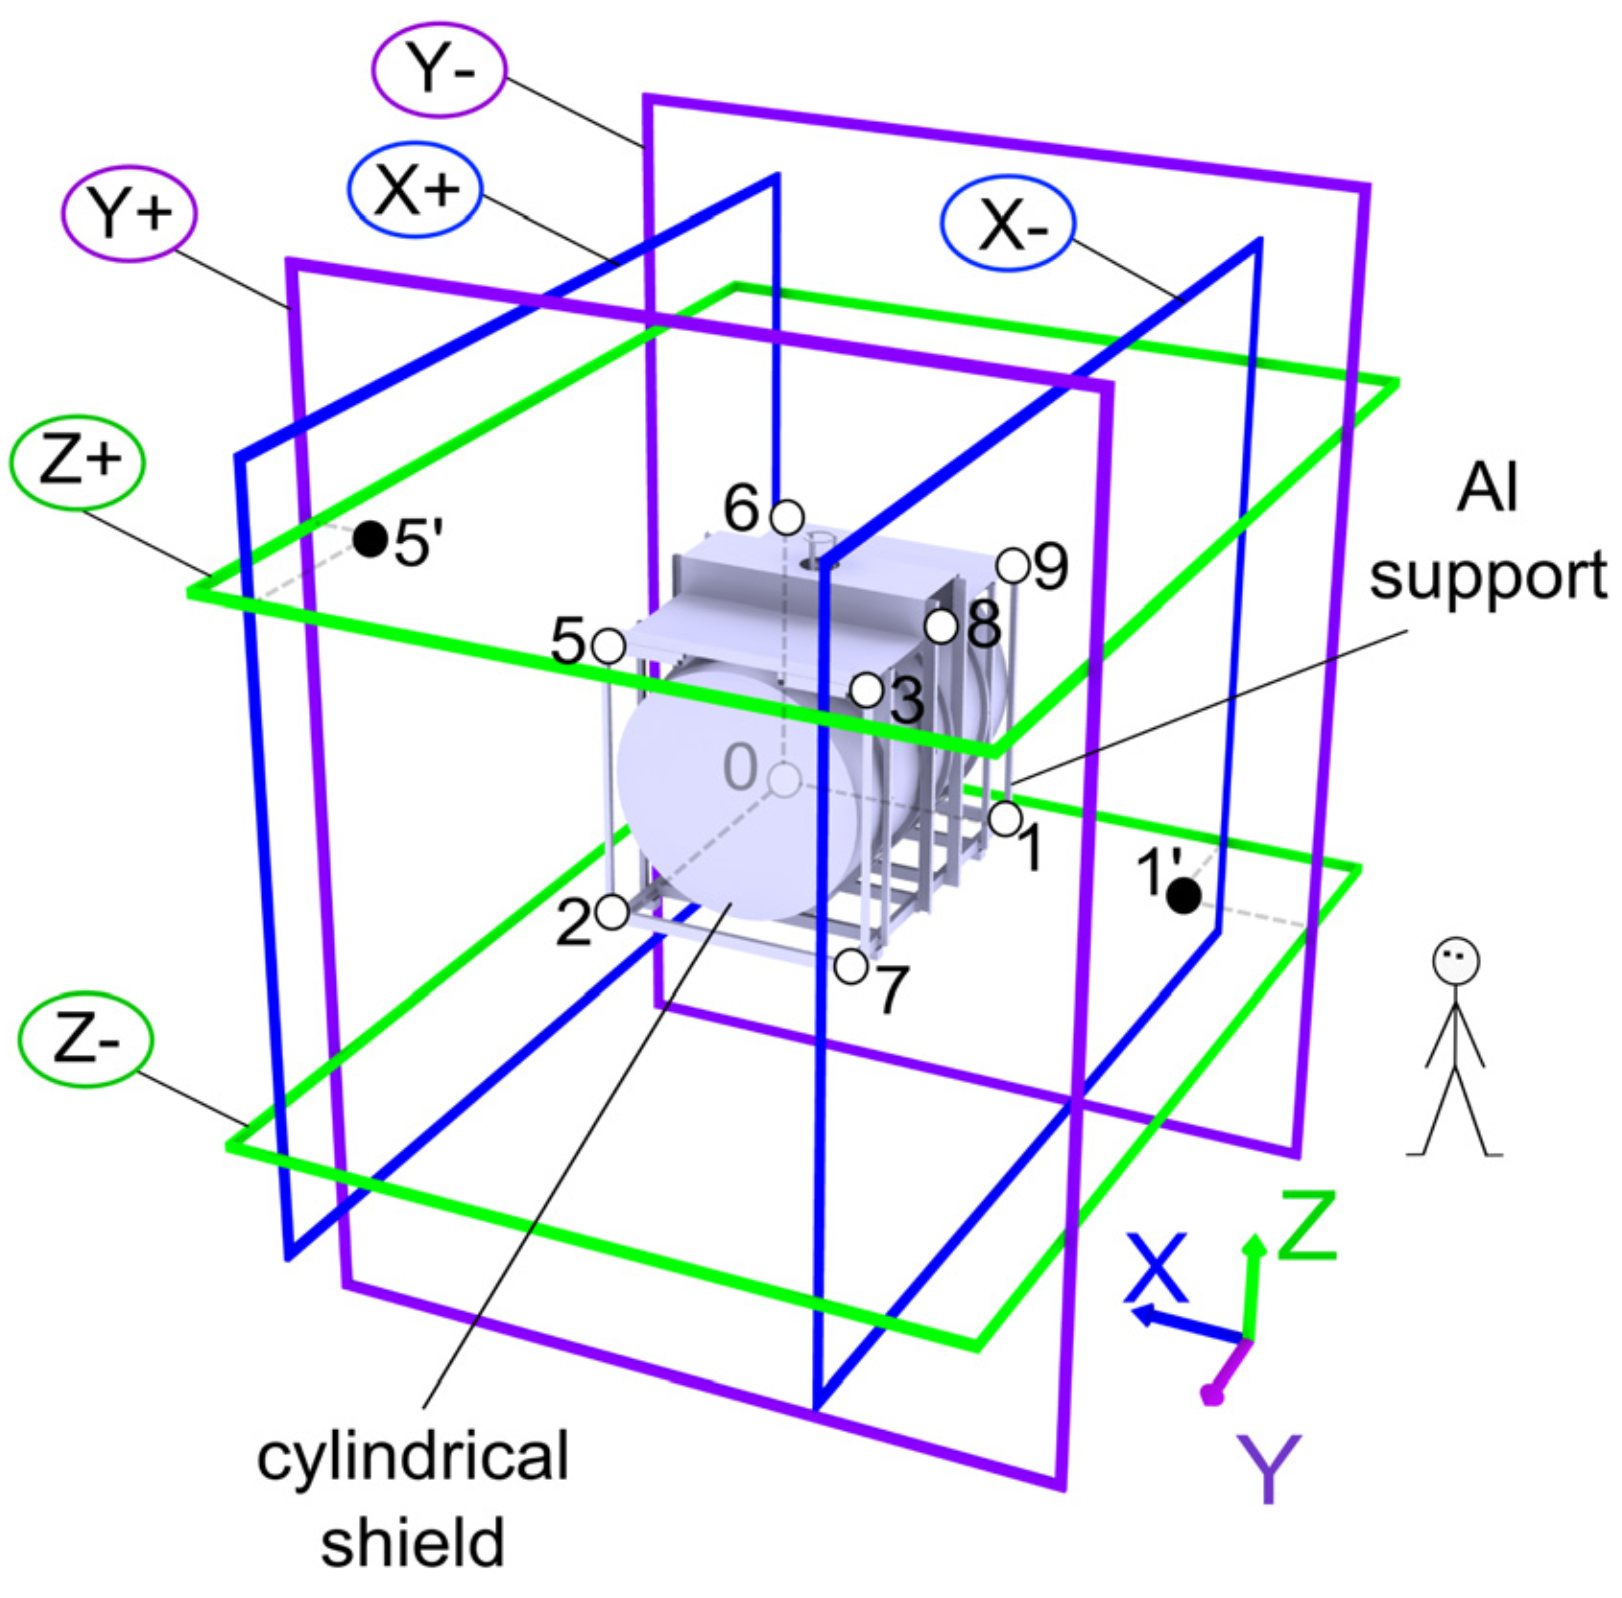
\includegraphics[width=.6\linewidth]{gfx/nEDM_SFC}
  \caption
  [Sketch of the nEDM SFC system.]
  {%FIXME directly copied from the SFC paper
Sketch of the SFC system consisting of six coils surrounding the Mu-metal magnetic shield of the nEDM spectrometer. The visible outermost layer of the cylindrical shield is mounted in its aluminum support structure.
The Helmholtz coil pairs are labeled (X+, X-),(X-, Y-) and (Z+,Z-). The coordinate system of the experiment is given at the lower right. Its origin is at the center of the magnetic shield. Three--axis fluxgates (open circles) are mounted on the aluminium support of the experiment and numbered according to the fluxgate nomenclature given in the text. The positions 10 and 50 (full circles) depict previous locations of fluxgates FG 1 and FG 5 referred to in Sec. VB. FG 4 is omitted as it was removed from the system after a sensor failure.}
  \label{fig:nEDM_SFC}
\end{figure}

The SFC system operates since 2013, attenuating the magnetic field by factor more than 5, even during ramping of nearby magnets.


\subsection{Design for n2EDM}

The volume is cubic.

The SFC system is going to be very large --- $\unit[6x6x6]{m^3}$. Elaborate designs, such as wires of variable length, or arbitrarily bended wires would be complicated to realise in such scale.

Moreover, the system is going to enclose the whole apparatus.
Super crucial --- many coils on the same surface 3 for the first order compensation, but then 9 for gradients. That is already 12 coils. If one only restrict oneself to a surface, it is guaranteed to end up with it densely covered with wires. In this approach the geometry is limited by design.

Mention, that the \micro-metal presence does not disturb much, as it is already placed in a small field.


Design goals / challenges:
\begin{enumerate}
  \item Better shielding factor. Attenuation by a factor of 50 in the whole volume of the shield. The design goal has been set to reach at most 2\% of the ambient magnetic field in the
  whole volume of the experiment. In \unit[50]{\micro T} this corresponds to a nice value of \unit[1]{\micro T}.
  \item Very large fiducial volume --- due to spatial constrains of the experimental site --- biological shielding. PUT IMAGE!!! Not only is the compensation expected to be better, but also provide a much larger volume. Next version of the experiment --- much larger.
  \item As is nEDM --- many coil system. But orthogonal, or at least close to one. Three coils for compensating the three homogeneous components of the magnetic field. Then 9 for gradients. The strongest fields are low--order, and only these require strong compensation coils (thick wires, big and expensive power supplies). The higher--order coils may be constructed with thinner wires and cheaper power supplies.
  Additionally, this makes the control of the system simpler.
  This also states the problem better. One has to design and construct coils that create homogeneous field in the volume occupied by the shield. Maybe elaborate more on the field decomposition!
  \item Coil tailored for the specific magnetic environment of the n2EDM site. Coils tailored for nearby magnets.
\end{enumerate}


\section{Prototype}
A comprehensive setup for prototyping magnetic field related systems for n2EDM has been designed and is, as of today, under construction. Its main part is a scaled--down model of the outermost layer of n2EDM µ-metal shield. Design of a degaussing and SFC systems for the setup is ongoing. In the future the setup can host also a prototypes of an internal magnetic field mapper, a main holding--field coil and, possibly, other systems.

\subsection{Maps}

\section{Potential problems}
\begin{enumerate}
  \item The numerical problem of subtracting numbers.
  \item The discretisation is happening twice --- first is the division into tiles. Then the current in the solution needs to be discretised too.
\end{enumerate}
